%\documentclass{article}
\documentclass[11pt,a4paper]{article}
%\documentclass[twoside, 11pt,a4paper]{article}
% Damit die Verwendung der deutschen Sprache nicht ganz so umst\"andlich wird,
% sollte man die folgenden Pakete einbinden: 
%\usepackage[latin1]{inputenc}% erm\"oglich die direkte Eingabe der Umlaute 

\usepackage{enumitem} % Anpassung der Klammern in enumerate
\usepackage[utf8]{inputenc}
\usepackage[T1]{fontenc} % das Trennen der Umlaute
%\usepackage{ngerman}[babel] 
\usepackage[english,ngerman]{babel} %Version in meinem Numerik Vortrag
\usepackage{caption}[2011/11/10]


% --------Figures ------------------------------------------------------
\newcommand{\figsource}[1]{%
	\addtocounter{figure}{-1}
	\captionlistentry{source: #1}
}
\newcommand{\source}[1]{\caption*{\hfill Quelle: {#1}} }
% -----------------------------------------------------------------------

\usepackage{mathtools}
\mathtoolsset{centercolon} % schönere Version für :=
% ----------------Headings font -----------------------------------------------------------------------
%\usepackage{titlesec}  %
%\titleformat{\section}[hang]{
%	\usefont{T1}{qhv}{b}{n}\selectfont} % "qhv" - TeX Gyre Heros, "b" - bold
%{} 
%{0em}
%{\hspace{-0.4pt}\Large \thesection\hspace{0.6em}}



%-------------------------------------------------------------------------------------------------------

% --- Algorithmen ---------------------------

\usepackage{algorithm} 
\usepackage{algorithmic}
%\usepackage[ruled,algosection,algo2e]{algorithm2e} 
\renewcommand*{\listalgorithmname}{Algorithmenverzeichnis} 
%\usepackage{algpseudocode}

%\addcontentsline{toc}{section}{List of algorithms}
% ------------------------------------------------

% --- Include .txt-files ---------------------------
%\usepackage{verbatim}
\usepackage{fancyvrb}

% -----------------------------------------------------



\usepackage[multiple]{footmisc}
\usepackage{pythontex} % \inputpygments{python}{file_1.py}
%\usepackage{caption}
\usepackage{verbatim}
\usepackage{subcaption}
\usepackage{amssymb}  

\usepackage{amsmath}
\DeclareMathOperator*{\argmax}{arg\,max}
\DeclareMathOperator*{\argmin}{arg\,min}

\usepackage{amsthm}
\usepackage[hidelinks]{hyperref}
\usepackage{graphicx}
\graphicspath{{images/}} %import images from follder "images

%\usepackage{apacite} %bibliography file
\pagenumbering{arabic}
\usepackage[labelfont=bf]{caption}
%\usepackage{ntheorem}
\usepackage{tabto}  
\usepackage{appendix}  
\usepackage[multiple]{footmisc} %multiple footnotes
%\newcommand\mytab{\tab \hspace{1cm}}
%\theoremstyle{break}

%%% ------------ Kopf- und Fußzeile
% https://esc-now.de/_/latex-individuelle-kopf--und-fusszeilen/?lang=de
\usepackage[headtopline,headsepline]{scrpage2}
\pagestyle{scrheadings}
\renewcommand{\headfont}{\scriptsize}

\clearscrheadfoot
\ofoot{\pagemark}

\ohead{\headmark}
\automark[subsection]{section}

% Linien

\setheadtopline{0pt}
\setheadsepline{.5pt}

% Keywords command
\providecommand{\keywords}[1]
{
	\small	
	\textbf{\textit{Keywords---}} #1
}
%%% -----------Theorem, Sätze, Beweise ----------------------------------------
%vgl. O.C.Schnürer FA Skript
%\usepackage{amsthm}

\def\emph#1{\textit{#1}}

%\newtheorem{theorem}{Theorem}[chapter]
\newtheorem{theorem}{Theorem}[subsection]
\newtheorem{lemma}[theorem]{Lemma}
\newtheorem{satz}[theorem]{Satz}
\newtheorem{proposition}[theorem]{Proposition}
\newtheorem{corollary}[theorem]{Korollar}

%\theoremstyle{definition}
\newtheorem{definition}[theorem]{Definition}
\newtheorem{example}[theorem]{Beispiel}
\newtheorem{beispiel}[theorem]{Beispiel}
\newtheorem{beispiele}[theorem]{Beispiele}
\newtheorem{xca}[theorem]{\"Ubung}
\newtheorem{notation}[theorem]{Notation}

\newtheorem{aufgabe}{Aufgabe}[section]
%\theoremstyle{remark}
\newtheorem{remark}[theorem]{Bemerkung}
\newtheorem{bemerkung}[theorem]{Bemerkung}
\newtheorem{herleitung}[theorem]{Herleitung}

%\numberwithin{section}{chapter}
%\numberwithin{equation}{chapter}
\numberwithin{equation}{section}
%----------------Titlepage -----------------------------------------------
\usepackage{pbox}


% -------------------------------------------------------------------------

%\renewcommand*{\proofname}{Beweis}
%%% -----------------------------------------------------------
% Python code einfügen:
\usepackage{listings}
\usepackage{xcolor}

\definecolor{codegreen}{rgb}{0,0.6,0}
\definecolor{codegray}{rgb}{0.5,0.5,0.5}
\definecolor{codepurple}{rgb}{0.58,0,0.82}
\definecolor{backcolour}{rgb}{0.95,0.95,0.92}

\lstdefinestyle{mystyle}{
	backgroundcolor=\color{backcolour},   
	commentstyle=\color{codegreen},
	keywordstyle=\color{magenta},
	numberstyle=\tiny\color{codegray},
	stringstyle=\color{codepurple},
	basicstyle=\ttfamily\footnotesize,
	breakatwhitespace=false,         
	breaklines=true,                 
	captionpos=b,                    
	keepspaces=true,                 
	numbers=left,                    
	numbersep=5pt,                  
	showspaces=false,                
	showstringspaces=false,
	showtabs=false,                  
	tabsize=2
}

\lstset{style=mystyle}
%\usepackage[nottoc,numbib]{tocbibind} %add bibliography to table of contents

%% --------------glossary -----------------------------

\usepackage[toc]{glossaries}

\newglossaryentry{llrp}
{
	name=Layer-wise Relevance Propagation,
	description={Verfahren zur Relevanzverteilung auf einzelne Neuronen eines Neuronalen Netzwerkes}
}

\newglossaryentry{latex}
{
	name=latex,
	description={Is a mark up language specially suited 
		for scientific documents}
}
\newacronym{lrp}{LRP}{Layer-wise Relevance Propagation}
\newacronym{dtd}{DTD}{Deep Taylor-Decomposition}
\newacronym{nn}{NN}{Neuronales Netzwerk}

\makeglossaries

%%-------------bibfile---------------------------------
\usepackage{cite}

%%%%%%%%%%%%%%%%%%%% -------------------------------------------------
%\newcommand*{\captionsource}[2]{%
%	\caption[{#1}]{%
%		#1%
%		\\\hspace{\linewidth}%
%		\vspace{5cm}\text{Quelle:} #2%
%	}%
%}


%\begin{figure} [ht]
%	\centering
%	\caption{text}
%	\captionsource{Caption}{asdasdasdasda}
%	\label{fig:gliederung}
%\end{figure}
%\newtheorem{theorem}{Theorem}

\title{\line(1,0){350}\\Untersuchung \& Entwicklung \\von Ansätzen zur Detektion von Poisoning-Angriffen\\\line(1,0){350}\\
	Master-Arbeit}
\author{
	Lukas Schulth\\
	\texttt{lukas.schulth@uni.kn}
}

\date{1. Oktober 2021}

\begin{document}

	\begin{titlepage}
		\thispagestyle{empty} 
		\begin{figure}
			\centering
			\begin{minipage}{0.45\textwidth}
				\centering
				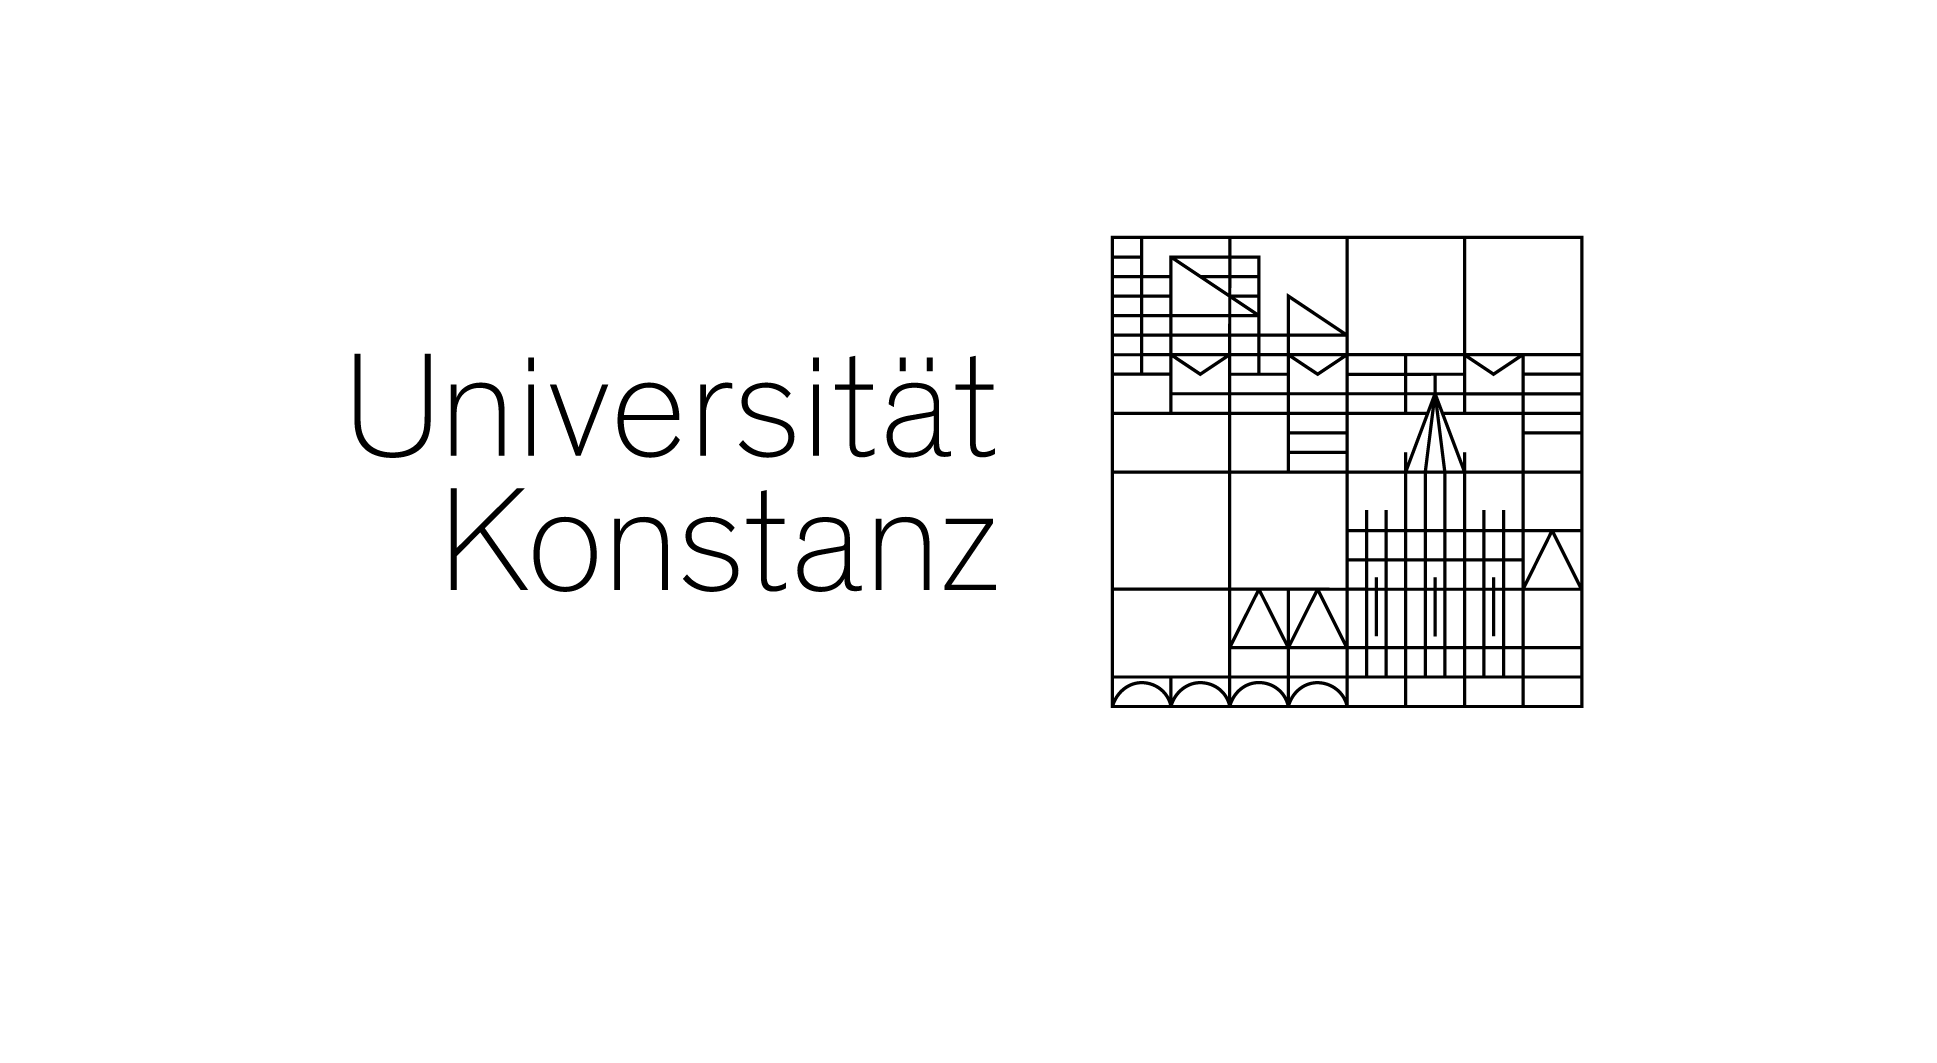
\includegraphics[width=1.2\textwidth]{logounikn} % first figure itself
				
			\end{minipage}\hfill
			\begin{minipage}{0.45\textwidth}
				\centering
				
\includegraphics[width=0.9\textwidth]{bsi_logo} % second figure itself
				
			\end{minipage}
		\end{figure}
		\centering
		\vspace{1cm}
		{\scshape\LARGE Universität Konstanz\\
			\large Fachbereich Mathematik und Statistik\\
			 \& \\ \LARGE Bundesamt für Sicherheit in der Informationstechnik \par}
		\vspace{1cm}
		{\scshape\Large Masterarbeit zum Thema:\par}
		\vspace{0.5cm}
		{\Huge \bfseries Untersuchung \& Entwicklung von Ansätzen zur Detektion von Poisoning-Angriffen\par} %corher wars in \huge, das sah auch nicht so schlecht aus
		\vspace{0.5cm}
		vorgelegt von \par
		\vspace{0.5cm}
		{\Large Lukas Schulth\\
			\texttt{lukas.schulth@uni.kn}\par}
		%\vfill
	
		
		
	
	
		\vspace{1cm}
		unter der Betreuung von\par
		\centering
		\begin{figure}[h]
			
			\makebox[1 \textwidth][c]{   
				\begin{tabular}{ll}
					\pbox{20cm}{Erstkorrektor: \\
						Herr Prof. Dr. Johannes Schropp \\ \texttt{johannes.schropp@uni.kn}} 
					& \pbox{20cm}{Zweitkorrektor:\\
						Herr Prof. Dipl.-Ing. Markus Ullmann\\
						\texttt{markus.ullmann@bsi.bund.de}} \\ 
					&\\
					\pbox{20cm}{Herr Dr. Christian Berghoff \\ \texttt{christian.berghoff@bsi.bund.de}} 
					& \pbox{20cm}{Herr Matthias Neu \\ \texttt{matthias.neu@bsi.bund.de}}
					
				\end{tabular}
			}
		\end{figure}
		%\vfill
		%\vspace{0.25cm}
		% Bottom of the page
		{\large 1. Oktober 2021}
	\end{titlepage}
	
	
		
	\selectlanguage{english}
	\begin{abstract}english\end{abstract}
	\selectlanguage{ngerman}
	\begin{abstract}deutsch\end{abstract}
	TODO:
	\begin{itemize}
		\item Algorithmen aufschreiben kmeans

	\end{itemize}
	\keywords{one, two, three, four}
	\newpage
	%\thispagestyle{empty} 
	\listoffigures
	
	\listoftables
	
	\lstlistoflistings
	
	\listofalgorithms
	\newpage
	\tableofcontents
	\newpage
	\section{Einführung}
	Allein für Deutschland wird erwartet, dass mit Dienstleistungen und Produkten, die auf dem
	Einsatz von Künstlicher Intelligenz (KI) basieren, im Jahr 2025 Umsätze in Höhe von 488 Milliar­
	den Euro generiert werden – damit würde ein Anteil von 13 Prozent am Bruttoinlandsprodukt
	erreicht. Dabei ist die Erklärbarkeit von Entscheidungen, die durch KI getroffen werden, in
	wichtigen Anwendungsbranchen eine Voraussetzung für die Akzeptanz bei den Nutzenden, für
	Zulassungs- und Zertifizierungsverfahren oder das Einhalten der durch die DSGVO geforderten
	Transparenzpflichten. Die Erklärbarkeit von KI-Produkten gehört damit, zumindest im europäi-
	schen Kontext, zu den wichtigen Markterfolgsfaktoren.[STudieErklärbareKI]
	
	
	
	
	RIght to be forgottten,  General Data Protection Regulation (GDPR) in
	the European Union [5], \url{https://arxiv.org/pdf/2003.04247.pdf}, 5: G. D. P. Regulation, “Regulation (eu) 2016/679 of the
	european parliament and of the council of 27 april 2016
	on the protection of natural persons with regard to the
	processing of personal data and on the free movement
	of such data, and repealing directive 95/46,” Official
	Journal of the European Union (OJ), vol. 59, no. 1-88,
	p. 294, 2016.
	
	Datengewinnung(LRP)
	Datenverarbeitung(kMeans, Gromov Wasserstein)
	Pweave\footnote{\url{https://mpastell.com/pweave/}}
	
	A Complete List of All (arXiv) Adversarial Example Papers \footnote{\url{https://nicholas.carlini.com/writing/2019/all-adversarial-example-papers.html}}
	\\
	In sicherheitskritischen Anwendungsgebieten ist die Erklärung für das Zustandekommen einer Entscheidung genauso wichtig wie die Entscheidung selbst\cite{LRP_DNN}.
	
	Clustering auf Datenpunkten direkt(~50 Prozent = raten), Clustering auf Aktivierungen gut geeigneter Netzwerkschichten. Clustering auf den Heatmaps der verdächtigen Klasse.\\
	\\
	
	Clustering auf unterschiedlichen Repräsentationen der Bilder:
	\begin{itemize}
		\item Clustering direkt auf den Bildern\\
		\item Clustering auf den Activations einer Netzwerkschicht(Im Paper \cite{AC} wird die vorletzte Schicht benutzt)
		\item Clustering auf den Heatmaps
	\end{itemize}
	In \autoref{chapter_nn} geben wir eine kurze Einführung in Neuronale Netzwerke und stellen die untersuchten Modelle vor. \autoref{chapter_poisoningattacks} führt in die unterschiedlichen Möglichkeiten eines Poisoning-Angriffs auf Neuronale Netzwerke ein. \autoref{chapter_xai} gibt eine kurze Übersicht über den Bereich der Erklärbaren Künstlichen Intelligenz, wobei ein Beispiel eines Verfahrens, die sogenannte Layer-wise Relevanz Propagation ausführlich in \autoref{chapter_lrp} vorgestellt wird. Kern der Arbeit bildet \autoref{chapter_algorithm}, wo wir zu Beginn die grundlegenden Bestandteile des Algorithmus zur Detektion von Poisoning-Angriffen auf Neuronale Netzwerke erklären, bevor die experimentellen Ergebnisse in \autoref{chapter_results} ausführen. Ein Vergleich mit anderen Detektionsverfahren wird in \autoref{chapter_comparisons} durchgeführt.
	
	AI \footnote{\url{https://builtin.com/artificial-intelligence?__cf_chl_captcha_tk__=pmd_ZUF1SDojKVlMszuDEU4Rp_4q3PfPzuXH3h7GVdvGMu8-1629552213-0-gqNtZGzNAxCjcnBszQhR}}
	\section{Neuronale Netzwerke} \label{chapter_nn}
	Wir betrachten ein \gls{nn}, dass die Funktion $f_{\theta}:\mathbb{R}^n \to\mathbb{R}$, mit $\theta = (w_{il}, b_{il})$ beschreibt. 
	i: Schicht
	l: Neuron in der Schicht
	w: Gewichte 
	b: Bias
	g: nichtlineare Akivierungsfunktion
	Architektur,
	Modell
	Pre-Activations(lokal, global): $z_{ij} = x_i*w_{ij}$
	$z_j = \sum_iz_{ij} + b_j$
	
	Vorschrift/aktivierungen: $x_j = g(z_{ij})$
	
	
	Training;testing, Validation, Forward pass, backward pass
	SGD erklärt im Einführungsteil von \cite{BatchNormalization}
	
	fehlende Interpretierbarkeit
	
	ReLUs in den meisten Netzwerken
	
	Definition Klasse
	
	Supervised vs Unsupervised
	
	Dimensionality reduction and Visualisation
	Was ist die letzte/vorletzte Shickht? vgl. Ac
	
	Wir verwenden die Begriffe Bild und Datenpunkt äquivalent.
	\subsubsection{CNNS}
	s. MA Juliane Braunsmann (convolutions /cross correlations)
	Idee, Abstraktion, high level, low level features, bekannte Netzwerke\\
	
	Ausführliche Einführung stanford Kurs\cite{cnn_stanford}. Unterschied zu FC layers: 
	It is worth noting that the only difference between FC and CONV layers is that the neurons in the CONV layer are connected only to a local region in the input, and that many of the neurons in a CONV volume share parameters. However, the neurons in both layers still compute dot products, so their functional form is identical. Therefore, it turns out that it’s possible to convert between FC and CONV layers
	
	Starting with LeNet-5   [10], convolutional neural networks (CNN) have typically had a standardstructure – stacked convolutional layers (optionally followed by contrast normalization and max-pooling)  are  followed  by  one  or  more  fully-connected  layers.   Variants  of  this  basic  design  areprevalent in the image classification literature and have yielded the best results to-date on MNIST,CIFAR and most notably on the ImageNet classification challenge [9, 21].  For larger datasets suchas Imagenet, the recent trend has been to increase the number of layers  [12] and layer size [21, 14],while using dropout [7] to address the problem of overfitting.\cite{goingdeeperwithconvolutions}
	
	Softmax am Ende für Transformation in Probabilities.
	
	Netzwerk im Netzwerk \cite{cnn_architectures_stanford, goingdeeperwithconvolutions}
	
	\subsubsection{Besondere Schichten}
	Promotion Sebastian Lapuschkin
	
	\begin{itemize}
		\item \textit{BatchConv} besteht aus 
		\begin{lstlisting}[language=Python, caption=python-interner Aufbau einer BatchConv Schicht
		]
		nn.Conv2d(in_channels=in_channels, out_channels=out_channels, **kwargs)
		nn.BatchNorm2d(num_features=out_channels)
		nn.ReLU()
		\end{lstlisting}
		in genau dieser Reihenfolge
		Bem.: Nur für BatchNorm2d müsste man LRP implementieren, für Conv2d funktioniert das bereits.
	\end{itemize}
	
	Batch Normalization\footnote{\url{https://arxiv.org/pdf/1502.03167.pdf}}
	
	
	\subsubsection{Inception v3}
	Filter,
	In Klassischen feed forward Netzen wird Output der vorheigen layer ist input der nächsten layer
	
	Jetzt: Inception Block: Previous layer input, 4 operations in parallel, concatenation,1x1 conv -> lower dimension -> less computational cost
	
	Intermediate classifiers: kommt aus multitask learning. Eigentlich eine Möglickeit gegen vasnishing gradients
	
	\subsubsection{VGG16}
	VGG16 is a convolutional neural network model proposed by K. Simonyan and A. Zisserman from the University of Oxford in the paper Very Deep Convolutional Networks for Large-Scale Image Recognition. The model achieves 92.7\% top-5 test accuracy in ImageNet, which is a dataset of over 14 million images belonging to 1000 classes. It was one of the famous model submitted to ILSVRC-2014. It makes the improvement over AlexNet by replacing large kernel-sized filters (11 and 5 in the first and second convolutional layer, respectively) with multiple 3×3 kernel-sized filters one after another. VGG16 was trained for weeks and was using NVIDIA Titan Black GP’s.%\cite{vgg16_neurohive} \cite{vgg16_architecture}
	
	\subsection{Datensatz}
	GTSRB\footnote{\url{https://benchmark.ini.rub.de/gtsrb_dataset.html}}
	
	Für die Poisoning-Angriffe auf verschiedene neuronale Netzwerke benutzen wir
	den Datensatz German Traffic Sign Recognition Benchmark 1 . Dieser besteht
	aus 52.001 Bildern von Verkehrsschildern aus 43 verschiedenen Kategorien der
	Pixelgröße 32x32. Etwa 75 Prozent der Bilder wird für das Training, die ande-
	ren 25 Prozent für das Testen benutzt. Der Datensatz wurde ursprünglich in
	einem Wettbewerb auf der International Joint Conference on Neural Networks
	(IJCNN) im Jahr 2011 benutzt. Die Bilder sind aus aus einer Videosequenz
	herausgeschnitten. Deshalb befinden sich in einer Klasse jeweils immer meh-
	rere Bilder desselben Verkehrsschildes zu unterschiedlichen Zeitpunkten. Auf-
	nahmen desselben Verkehrsschildes kommen nicht übergreifend in Training-,
	Validierung- oder Testdatensatz vor.
	Verkehrsschild
	\begin{table}[h]
		\begin{tabular}[h]{c|c}
			Verkehrsschilder & Anzahl an Bildern \\ \hline
			’Zulässige Höchstgeschwindigkeit: 20km/h’& 180 \\
			’Zulässige Höchstgeschwindigkeit: 30km/h’ & 1980 \\
			’Zulässige Höchstgeschwindigkeit: 50km/h’	& 2010 \\
			’Zulässige Höchstgeschwindigkeit: 60km/h’	& 1260 \\
			’Zulässige Höchstgeschwindigkeit: 70km/h’	& 1770 \\
			’Zulässige Höchstgeschwindigkeit: 80km/h’	&1650 \\
			’Halt! Vorfahrt gewähren’					&	690
		\end{tabular}
		\label{tab:Auswahl_Datensatz}
		\caption{Für einen Poisoning-Angriff interessante Klassen und die zugehörige Anzahl an Bildern.}
	\end{table}
	
	
	
	
	
	
	
	
	In \autoref{tab:Auswahl_Datensatz} sind einige Klassen der Verkehrsschilder und deren An-
	zahl im Datensatz aufgelistet, die für einen Poisoning-Angriff interessant sein
	könnten. Die Anzahl der Schilder ’Halt! Vorfahrt gewähren’-Schilder im Trainingssatz beträgt etwa 690 Aufnahmen. Diese wurden von insgesamt nur 24 verschiedenen ’Halt! Vorfahrt gewähren’-Schildern aufgenommen. Da beim Erstel-
	len der korrumpierten Daten auch immer das Bild aus der angegriffenen Klasse
	in die Zielklasse verschoben wird, wird die Anzahl der in der Ursprungsklasse verbleibenden Daten abhängig vom Anteil an korrumpierten Daten kleiner.
	Wir werden uns deshalb im Folgenden mit Angriffen auf die Klasse ’Zulässige
	Höchstgeschwindigkeit: 50 km/h’ beschäftigen, da sie die höchste Anzahl an
	Daten aufweist.
	
	
	\section{Poisoning-Angriffe} \label{chapter_poisoningattacks}
	Gute BEschreibung in 3.Method \url{https://arxiv.org/pdf/1910.00033.pdf}
	Mithilfe eines manipulierten Datensatzes wird das Netzwerk manipuliert, sodass die Entscheidung des Netzwerkes abhängig von einem Auslöser ist.
	
	\noindent \textbf{Wer wird wie angegriffen?}: Der Angreifer erstellt einen Datensatz, sodass in den Netzwerken, die auf diesem Datensatz trainiert werden eine Hintertür implementiert wird. Damit ergibt sich die Annahme, dass der Angreifer volle Kontrolle über den Datensatz hat und somit Datenpunkte entfernen oder hinzufügen kann.
	
	Was passiert, wenn der Angreifer keinen Zugriff auf die Modell-Architektur hat? Transfer-Learning? 
	
	\noindent \textbf{Anbringen des Auslösers}
	\subsection{Standard Poisoning-Angriffe}
	Wir wollen Schilder der Klasse 50kmh absichtlich falsch als 80kmh. Wir wählen diese beiden Klassen aufgrunde der Größe beider Klassen(s. Aufstellung in Praktikumsbericht). Stoppschildklasse ist wohl vergleichsweise ze8imlich klein.\\
	
	Dazu fügen wir auf den 50er Schildern einen Sticker ein und ändern das Label auf 80.
	Label-Consistent
	Backdoor Attacks
	Für die Bewertung, wie erfolgreich ein Angriff war, fügen wir in jedem Bild der 50er Klasse im Testdatensatz einen Sticker ein und messen, wie groß der Anteil der 50er Schilder ist, die als 80er Schild klassifiziert werden.\\
	
	\noindent \textbf{CH- und Backdoor-Artefakte}:\\
	In \cite{imagenet_unhansed_v2} wird wie folgt zwischen Clever Hans- und Backdoor-Artefakten unterschieden. In beiden Fällen wird rechts oben im Bild ein grauer 3x3 Sticker eingefügt.
	Bei CH geschieht dies bei $25 \%$ der "airplane"-Klasse. Bei Backdoor-Artefakten werden $10 \%$ aller Bilder korrumpiert. Im zweiten Fall wird das entspechende Label abgeändert. Dies entspricht dann einem Standard- bzw. Clean-Label-Poisoning-Angriff. (Wie git funktioniert der CLPA/CH hier ohne die Bilder vorher schlechter zu machen? TODO: Vergleich mit \cite{labelconsistent}). In \cite{imagenet_unhansed_v2}, Kapitel 2.1 wird auch auf die Methode der Spektralen Signatur \cite{spectral_signatures} eingegangen, die zur Detektion genutzt wird. Diese eignet sich wohl sehr gut für die Backdoor-Attacks, aber nur schlecht für die CH-Artefakte.
	
	
	\subsection{Label-konsistente Poisoning-Angriffe}
	Bei den vorheringen Standard-Angriffen war es der Fall, dass das Label und das entsprechende Bild nicht mehr zusammenpassen. Ein händisches Durchsuchen des Datensatz (wenn auch sehr aufwendig) könnte damit ebenfalls zur Detektion eines Angriffs führen.\\
	Eine deutlich schwieriger zu detektierende Art von Poisoning-Angriffen sind sogenannte Label-konsistente Angriffe, bei denen genau diese Schwachstelle eliminiert ist, d.h. Label und Bild passen wieder zueinander, während der Angriff noch immer erfolgreich funktioniert. Es ist das Ziel, ein Bild zunächst so zu modifizieren, dass es für das menschliche Auge noch immer zur entsprechenden Klasse gehört,für das Neuronale Netzwerk aber so schwierig zu klassifizieren ist, dass sich das Netzwerk eher auf den Auslöser anstatt auf das ursprüngliche Bild verlässt. Im Anschluss wird wieder ein Auslöser eingefügt.\\
		
	In \cite{labelconsistent} werden zwei Verfahren vorgestellt, die die Klassifikation einzelner Bilder erschweren. Das erste Verfahren besteht aus einer Einbettung in einen niedrig-dimensionalen Raum, das auch bei Autoencodern, etc. verwendet wird TODO.
	
	Beim zweiten Verfahren wird ein sogenannte Projizierter Gradienten-Abstieg-Angriff durchgeführt.\\
	Dabei wird ein Adversarialer Angriff in leicht abgewandelter Form genutzt, um das Netzwerk zu stören. Bei Adversarialen Angriffen wird ein Netzwerk im Unterschied zum Poisoning-Angriff, bei dem der Angriff während des Trainings stattfindet, nach dem Training angegriffen. Dazu wird eine natürliche Netzwerkeingabe leicht gestört, sodass diese vom Netzwerk falsch klassifiziert wird. Diese Störungen lassen sich auch von einer Architektur oder sogar einem Modell auf andere übertragen \cite{szegedy2013intriguing, papernot2016transferability}.
	%TODO: Unterschied zw. Klassifizierung und Klassifikation
	Für diese Art von Angriff werden die adversarialen Angriffe und ihre leichte Übertragbarkeit auf andere Architekturen und Modelle so benutzt, dass es bereits während des Trainings zu falschen Klassifikationen kommt.\\
	Für unser erstes trainiertes Netzwerk $f_\theta$ mit Verlustfunktion $\mathcal{L}$ und einem Eingabe-Paar $(x,y)$, konstruieren wir die modifzierte Version von $x$ als
	\begin{equation}
		x_{adv} = \argmax_{||x'-x||_p \leq \varepsilon}{\mathcal{L}(x',y,\theta},
	\end{equation}
	
	für $p >1 $ und $\varepsilon > 0$. Dieses Optimierungsproblem wir mit einem Projizierten Gradienten-Verfahren \cite{madry2017towards}. Details dazu finden sich in \autoref{param_attacks}. Im Unterschied zu \cite{labelconsistent} ändern wir nur Bilder im Datensatz ab und fügen nicht zusätzlich zum Original $x$ auch $x_{adv}$ hinzu. Damit ändert sich die Anzahl an Datenpunkten durch den Angriff nicht.
	
	Für das anschließende Einfügen des Auslöser ergeben sich die folgenden Optionen:
	\begin{itemize}
		\item Der im Standard-Angriff verwendete Sticker
		\item Ein Amplitudensticker: Dabei wird im rechten unteren Eck des Bildes ein 
		\item Amplitudensticker 4 fach
		\item In die Mitte verschobene Amplitudensticker
	\end{itemize}
	RGB auf jedem Kanal in der range von [0,255]
	0 entspricht weiß, 255=schwarz
	Da die zweite Möglichkeit als deutlich erfolgreicher angegeben wird, beschränken wir uns auf diese Angriffe basierend auf einem Projizierten Gradienten-Abstieg.
	amp=16,32,64,255
	Wir gehen zunächst davon aus, dass der Angreifer volle Kontrolle über den Datensatz und das Netzwerk besitzt.TODO: Angriff mit einem andere Netzwerk erstellen, als das angegriffene
	
	\subsection{Bewertung von Poisoning-Angriffen}
	
	Wann ist ein Angriff erfolgreich?\\
	Im Trainingsdatensatz werden im Fall des Standard-Angriffs alle Bilder mit dem Sticker versehen. Die Angriffserfolgsrate beschreibt nun den Anteil an Bildern der attackierten Klasse, die erfolgreich falsch klassifiziert wurden.\\
	
	Für die Label-konsistenten Angriffe werden im Test-Datensatz alle Bilder mit dem entsprechenden Auslöser versehen und es kann eine Erfolgsrate pro Klasse berechnet werden. Es ist zu beachten, dass für Angriffe, die mit einer reduzierten Amplitudenstärke durchgeführt werden, die Bilder im Test-Datensatz dennoch mit Auslösern mit voller Amplitudenstärke versehen werden. 
	
	\subsection{Verteidigungen}
	In diesem Kapitel beschäftigen wir uns mit gängigen Methoden zur Detektion von Poisoning-Attacks und geben am Ende einen kurzen Ausblick auf die Idee für einen neuen Ansatz.
	Wir wollen beide Arten von Poisoning-Angriffen erfolgreich detektieren. 
	
	\subsubsection{Referenzwert: kMeans(k=2)}
	Der einfachste Ansatz, um korrumpierte Datenpunkte zu erkennen, ist ein kMeans-Clustering, das direkt(bzw. nach einer Dimensionsreduktion) auf den Eingabedaten einer Klasse durchgeführt wird. Hierbei war auffällig, dass der Großteil der Daten als korrumpiert klassifiziert wurde. Für die Dimensionsreduktionen FastICA und PCA ergab sich eine Genauigkeit von etwa $66 \%$. Die FPR lag bei über 70 \%, die TPR bei ca. $50 \%$.
	Dieser Referenzwert w@article{szegedy2013intriguing,
		title={Intriguing properties of neural networks},
		author={Szegedy, Christian and Zaremba, Wojciech and Sutskever, Ilya and Bruna, Joan and Erhan, Dumitru and Goodfellow, Ian and Fergus, Rob},
		journal={arXiv preprint arXiv:1312.6199},
		year={2013}
	}
	urde für einen Sticker mit Seitenlänge 3 und $15 \%$ korrumpierten Daten durchgeführt.
	\subsubsection{Activation Clustering}
	
	
		Nehme Datensatz her
		Beim Standardangriff wollen wir Klasse 5 als Klasse 8 klassifzieren und fügen dazu Sticker der  
		
		
		Diese Idee der Verteidigung basiert auf der Annahme, dass bestimmte Schichten innerhalb des Netzwerkes die Entscheidung, dass ein Bild mit einem Auslöser falsch klassifiziert wird, sehr gut codieren. Für die Detektion der Hintertüren im Datensatz sollen nun genau diese Aktivierungen für ein Clustering herangezogen werden.
		Das Activation Clustering wird erstmalig in \cite{AC} vorgestellt und nutzt aufgrund experimenteller Untersuchungen stets die Aktivierungen der vorletzten Netzwerkschicht.
		Eine Kombination von Aktivierungen mehrere Schichten wäre ebenfalls denkbar.
				
		Ein Angriff ist erfolgreich, wenn eine große Anzahl an Datenpunkten der Ur-
		sprungsklasse, versehen mit einem Auslöser, der Zielklasse zugeordnet werden.
		Im Falle eines erfolgreichen Angriffs werden korrumpierte und nicht korrumpier-
		te Datenpunkte im Trainingsdatensatz derselben Klasse zugeordnet. Der Grund
		weshalb diese derselben Klasse zugeordnet werden, unterscheidet sich jedoch.
		Beim Activation Clustering wird nun angenommen, dass pro Klasse entweder
		korrumpierte und nicht korrumpierte Datenpunkte oder nur nicht korrumpierte
		Datenpunkte existieren. Deshalb werden die Aktivierungen der letzten verdeck-
		ten Schicht des Netzwerkes aus dem Netz extrahiert, nach ihren zugehörigen
		Klassen der Labels segmentiert, auf 10 Dimensionen reduziert und anschließend
		mit Hilfe des kMeans-Algorithmus geclustert. Das kleinere Cluster wird immer
		als der Anteil an verdächtigen Datenpunkten betrachtet. Die Idee ist es, dass
		die korrumpierten Datenpunkte, sofern welche existieren, alle in die eine und
		die nicht korrumpierten Datenpunkte in das andere Cluster aufgeteilt werden.
		Sind keine korrumpierten Datenpunkte vorhanden, so sollen beide Cluster un-
		gefähr dieselbe Anzahl an Datenpunkten erhalten.\\
		
		Wir werten die Qualität des Clusterings anschließend aus. Als Detektionsrate
		beschreiben wir die Genauigkeit des Clusterings auf den Trainingsdaten.
		
		Im folgenden Abschnitt werden Methoden vorgestellt, mit denen das resultierende Clustering auf die präsenz eines Angriffs untersucht werden kann. Dies ist notwendig, da in der Praxis ein Angriff zunächst erkannt und anschließend die korrumpierten Datenpunkte entfernt werden müssen. 
		
		\begin{remark}
			Das SPA benutz die Idee das innerhalb einer Klasse bezüglich unterschiedlicher Aktivierungen klassifiziert werden kann. Beim CLPA funktioniert das nicht mehr, denn: Hier passen jetzt auch die Aktivierungen der korrumpierten Bilder zur entsprechenden/untersuchten Klasse. Es ist also zu erwarten, dass das AC für CLPA nicht funktioniert.
		\end{remark}
	
		\subsection{Implementierung}
		Wir nutzen die python Implementierun in sklearn mit den Standard-Werten $n\_init=10$ und $max\_iter=300$
		
		
		\subsubsection{Methoden zur Untersuchung, ob ein Angriff vorliegt}
		\#TODO: Vergleich mit Fisher-Discriminant-Anaylsis/Ansatz in \cite{imagenet_unhansed_v1}
		Zur
		Bestimmung, ob eine Klasse korrumpierte Daten enthält, kann das Ergebnis
		des Clusterings mit den folgenden Methoden untersucht werden:\\
		
		\noindent \textbf@article{szegedy2013intriguing,
			title={Intriguing properties of neural networks},
			author={Szegedy, Christian and Zaremba, Wojciech and Sutskever, Ilya and Bruna, Joan and Erhan, Dumitru and Goodfellow, Ian and Fergus, Rob},
			journal={arXiv preprint arXiv:1312.6199},
			year={2013}
		}
		{Vergleich der relativen Größe:} Eine Möglichkeit, korrumpierte Datenpunkte
		zu erkennen, ist der Vergleich der relativen Größen der beiden Cluster. Laut [2]
		ist die relative Größe bei nicht korrumpierten Klassen ca. 50 Prozent, bei kor-
		rumpierten Daten und einem erfolgreichen Clustering würde die relative Größe
		dann dem prozentualen Anteil an korrumpierten Datenpunkten entsprechen.\\
		
		\noindent \textbf{Silhouette-Koeffizient:} Eine weitere Möglichkeit besteht darin, die Qualität
		des Clusterings mit Hilfe des Silhouette-Koeffizienten zu beschreiben. Dieser gibt
		an, wie gut ein Clustering zu den gegebenen Datenpunkten mit den entsprechen-
		den Labeln passt und ist wie folgt definiert: Sei das Ergebnis eines Clustering-
		Algorithmus mit verschiedenen Clustern gegeben. Zu einer Beobachtung $x$ im Cluster $A$ wir die Silhouette $s(x) = \frac{d(B,x)-d(A,x)}{max\lbrace d(A,x), d(B,x) \rbrace}$ definiert, wobei $d(A,x)  = \frac{1}{n_A -1}\sum_{a \in A, a \neq x}{d(a,x)}$ dem mittleren Abstand einer Beobachtung innerhalb einer Klasse zu allen anderen Beobachtungen dieser Klasse entspricht.
		Dabei steht $n_A$ für die Anzahl der Beobachtungen in Cluster A. $d(B,x) = \min_{C \neq A}d(C,x)$ beschreibt die Distanz von $x$ zum nächstgelegenen Cluster B. Der Silhouetten-Koeffizient $SC$ ist nun definiert als
		\begin{equation}
			SC = \max_k \tilde{s}(k),
		\end{equation}
		wobei $\tilde{s}(k)$ der Mittelwert der Silhoutten aller Datenpunkte im gesamten Datensatz ist. Damit ist der Silhouttenkoeffizient ein Maß dafür, wie gut ein Clustering für eine vorher fixierte Clusteranzahl $k$ zum Datensatz passt.\\
		
		\noindent \textbf{Exklusives Retraining:} Beim exklusiven Retraining wird das neuronale Netz
		von Grund auf neu trainiert. Das oder die verdächtigen Cluster werden beim
		erneuten Training nicht benutzt. Mit Hilfe des neu trainierten Netzes wer-
		den dann anschließend die vorenthaltenen, verdächtigen Cluster klassifiziert.
		Falls das Cluster Aktivierungen von Datenpunkten enthält, die zum Label des
		Datenpunktes gehören, erwarten wir, dass die Vorhersage des Netzwerks mit
		dem Label übereinstimmen. Gehören die Aktivierungen eines Datenpunktes im
		verdächtigen Cluster jedoch zu einer anderen Klasse als die durch das Label
		angedeutete Klasse, so sollte das Netzwerk den Datenpunkt einer anderen Klas-
		se zuordnen. Um nun zu entscheiden, ob ein verdächtiges Cluster korrumpiert
		oder nicht korrumpiert ist, wird wie folgt vorgegangen: Sei $l$ die Anzahl an Vor-
		hersagen, die zum Label des Datenpunktes passen. Sei $p$ die größte Anzahl an
		Vorhersagen, die für eine weitere Klasse $C$ sprechen, wobei $C$ nicht die Klas-
		se mit den Labeln des zu untersuchenden Clusters ist. Der Quotient $\frac{l}{p}$ gibt
		dann an, ob das Cluster korrumpiert ist oder nicht: Es wird ein Schwellenwert
		$T > 0$ gesetzt. Gilt $\frac{l}{p} < T$ , wurden mehr Datenpunkte einer anderen Klasse zu-
		geordnet und das Cluster wird als korrumpiert deklariert. Umgekehrt wird das
		verdächtige Cluster im Fall von $\frac{l}{p} > T$ als nicht korrumpiert/sauber eingestuft.
		
		
		\subsubsection{Entfernen von korrumpierten Datenpunkten}
	
	\noindent \textbf{AC für Label-konistente Poisoning-Angriffe:} Warum funktioniert Activation-Clustering hier nur schlecht oder gar nicht?: Wenn wir einen korrumpierten Trainingsdatensatz gegeben haben, gilt im Fall des Standard-Angriffs folgender Sachverhalt: Die angegriffene Klasse, die Klasse in der samples eingefügt wurden, besitzt die eine Gruppe an Bildern, die zu einer Aktivierung von einer anderen Klasse führen sollten, und die Gruppe an Bildern, die zu dieser Klasse gehören und zur Aktivierung genau dieser Klasse führen sollte.\\
	Im Fall des Label-konsistenten Poisoning-Angriffs, werden nun keine Label mehr getauscht, d.h. Bilder von der einen in die andere Klasse verschoben. Damit können die beiden Gruppen (korrumpiert, sauber) innerhalb einer Klasse nicht mehr anhand ihrer Aktivierungen unterschieden werden.\\
	Trotzdem ergibt sich ein Ansatz daraus, dass es innerhalb dieser Klasse verschiedene \glqq Strategien\grqq{}  gibt, die zur selben Klassifikation führen. Mithilfe des kmeans-Clustering basierend auf den Heatmaps sollen genau diese Strategien ausfindig gemacht werden, um die Bilder in korrumpiert und sauber zu unterteilen.
	
	\subsubsection{Heatmap Clustering}
	Im Unterschied zum Activation Clustering, bei dem die Aktivierungen der vorletzten Netzwerk-Schicht verwendet werden, ist nun hier die Idee, zu jedem Eingabebild eine Relevanzkarte zu erstellen, die für jeden Pixelpunkt angibt, wie wichtig dieser für die Klassifikation dieses Bildes ist. \\
	
	Für das Erstellen/Berechnen solcher Relevanzkarten/Heatmaps existieren mehrere Methoden, die zusammengefasst dem Bereich der Erklärbaren KI zugeordnet werden.
	Im folgenden Kaptiel wollen wir einen kurzen Überblick über verschiedene Methoden geben.
	
	
	\section{Erklärbare KI}
	 \label{chapter_xai}
	
	
	Unkritische Anwendiuungen benötigen keine Erklärbarkeit: z.B. NEtflix-Empfehlungen, Maschinelle Übersetzungen.
	
	Wichtig ist Erklärbarkeit aber z.B. in Sicherheitskritischen Bereichen. Modelle sollten nicht diskriminierend sein. Gesetzliche Regelung: DSGVO: Recht auf Erklärbarkeit. Wie kommt man von einem Blackbox-Modell zu einer Erklärung? Surrogat/Stellvertreter-Modell
	
	Modelle: (ante-hoc) LErne direkt ein white-box-system: Lineare Modelle, Regelsystem, Entscheidungsbäume.
	
	Beispiel: für Surrogat Lerne zu einem NN ein NEtscheidungsbaum.
	
	Lime: Erzeuge einzelne Datenerklärungen: Lokale Approximation
	
	Saliency Map: Welche Bildbereiche waren für die Entscheidung wichtig\footnote{\url{https://www.youtube.com/watch?v=y2d16er1Pfs}}
	Saliency Map (Pixel Attribution)\footnote{\url{https://christophm.github.io/interpretable-ml-book/pixel-attribution.html}}
	
	Lipton führt eine grundsätzliche Begriffserklärung ein \cite{lipton2018mythos}
	Erklärbarkeit vs. Interpretierbarkeit, youtube talk?!
	
	
	Den Kern von KI-basierten Anwendungen – womit hier im Wesentlichen Anwendungen des
	maschinellen Lernens gemeint sind – bilden immer die jeweils zugrundeliegenden KI-Modelle.
	Diese lassen sich in zwei Klassen einteilen: White- und Black-Box-Modelle. White-Box-Modelle,
	wie bspw. auf nachvollziehbaren Eingangsgrößen basierende Entscheidungsbäume, erlauben
	das grundsätzliche Nachvollziehen ihrer algorithmischen Zusammenhänge; sie sind somit
	selbsterklärend in Bezug auf ihre Wirkmechanismen und die von ihnen getroffenen Entscheidun-
	gen. Bei Black-Box-Modellen wie neuronalen Netzen ist es aufgrund ihrer Verflechtung und Viel-
	schichtigkeit in der Regel nicht mehr möglich, die innere Funktionsweise des Modells nachzu-
	vollziehen. Zumindest für die Erklärung von Einzelentscheidungen (lokale Erklärbarkeit) können
	dann jedoch zusätzliche Erklärungswerkzeuge eingesetzt werden, um nachträglich die Nachvoll-
	ziehbarkeit zu erhöhen. KI-Entwickler können für Entscheidungserklärungen je nach den
	konkreten Anforderungen auf etablierte Erklärungswerkzeuge zurückgreifen, bspw. LIME, SHAP,
	Integrated Gradients, LRP, DeepLift oder GradCAM, die allerdings Expertenwissen voraussetzen.
	Für die Nutzenden existieren bislang nur wenig gute Werkzeuge, die intuitiv verständliche Ent-
	scheidungserklärungen liefern (Saliency Maps, Counterfactual Explanations, Prototypen oder
	Surrogat-Modelle).
	
	\noindent \textbf{Transparenz: }
	Transparenz wird im Folgenden als eine Modelleigen-
	schaft behandelt. Ist die Transparenz eines Modells
	gegeben, so ist es unter der Annahme nachvollziehbarer
	Eingangsgrößen selbsterklärend 4 . Die Eigenschaft der
	Transparenz lässt sich weiter unterteilen in die drei un-
	terschiedlichen Ausprägungen der „Simulierbarkeit“, der
	„Unterteilbarkeit“ und der „Algorithmischen Transparenz“
	(Lipton 2016). Dabei wird in der Literatur häufig von einer
	hierarchischen Abhängigkeit ausgegangen (Arrieta et al.
	2019), sodass die Simulierbarkeit eines Systems dessen
	Unterteilbarkeit und dessen algorithmische Transparenz
	impliziert. Entsprechend begründet die Unterteilbarkeit
	eines Systems auch dessen algorithmische Transpa-
	renz. Folglich gilt ein Modell – unter der Annahme erklär-
	barer Eingangsdaten – bereits als transparent, wenn es
	lediglich die Eigenschaft der algorithmischen Transpa-
	renz erfüllt. Die höchste Transparenzstufe erreicht ein
	Modell, wenn es die Eigenschaft der Simulierbarkeit und
	somit auch die beiden anderen
	Eigenschaften erfüllt.
	
	Ein System ist simulierbar, wenn
	auch eine Person die Entschei-
	dungen des zugrundeliegenden
	Algorithmus in angemessener
	Zeit nachvollziehen kann oder
	könnte, indem sie die einzelnen
	Schritte, die zur Herbeiführung
	einer Entscheidung nötig sind,
	manuell durchführt.	
	
	Beispiel: Beim manuellen
	Durchlaufen unterschiedlicher
	Pfade eines nicht allzu großen
	Entscheidungsbaumes, der auf
	nachvollziehbaren Eingangsgrö-
	ßen beruht, kann eine Person in
	jedem Knoten selbst überprüfen,
	ob eine individuelle Eigenschaft
	von Eingangsdaten bzw. ein Attribut erfüllt ist oder nicht.
	Gibt es keine Attribute mehr zu prüfen, hat die Person
	ein „Blatt“ des Entscheidungsbaums erreicht, welches
	das Ergebnis repräsentiert. 
	
	\noindent \textbf{Erklärbarkeit: }Da Transparenz für diverse Modelle wie z. B. neuronale
	Netze nicht erreichbar ist, diese folglich nicht selbst-
	erklärend sind, kommt bei diesen das Konzept der „Er-
	klärbarkeit“ zur Anwendung. Dabei ist zwar in der Regel
	festgelegt, ob die Erklärbarkeit eine Entscheidung oder
	ein Modell betrifft. Wie eine konkrete Erklärung dabei
	ausgestaltet ist oder wieviel Erkenntnis sie der Zielper-
	son gewährt, bleibt dabei jedoch zunächst unbestimmt.
	Beim Beispiel der Bildverarbeitung mit neuronalen Net-
	zen spricht man etwa bereits von einer Erklärung einer
	Entscheidung, wenn bestimmte Bereiche im Eingabe-
	bild, die zur Klassifikation eines konkreten Objektes ge-
	führt haben, für die anwendende Person farblich hervor-
	gehoben werden. In diesem Fall wird nicht jeder einzelne
	Schritt des Algorithmus erklärt, sondern nur die für die
	Entscheidungsfindung bedeutsamsten Daten hervor-
	gehoben. Alternativ kann eine Erklärung auch durch eine
	textliche Beschreibung repräsentiert werden, z. B. „Auf
	diesem Bild ist ein Hund abgebildet, da vier Beine, eine
	Schnauze, Fell und ein Schwanz erkannt wurden.“
	
	Grundsätzlich wird zwischen zwei Arten von Erklärungen unterschieden:
	
	\begin{itemize}
		\item Erklärungen von Einzelentscheidungen bzw. Ent-
		scheidungserklärungen, die dabei helfen, individuelle,
		datenbezogene Entscheidungen konkret nachzuvoll-
		ziehen (sogenannte lokale Erklärbarkeit oder Daten-
		erklärbarkeit).
		\item Erklärungen von Modellen bzw. Modellerklärungen,
		die dabei helfen, Wirkzusammenhänge von KI-Mo-
		dellen zu begreifen (sogenannte globale Erklärbarkeit
		oder Modellerklärbarkeit), z. B. lineare oder allgemein
		funktionale Zusammenhänge zwischen Eingangs-
		und Ausgangsgrößen.
	\end{itemize}

In den folgenden beiden Abschnitten stellen wir einige der bekanntesten Methoden aus beiden Bereichen vor.


	\noindent \textbf{text}
	\subsection{Lokale Methoden}
	
	Andere Aufteilung der lokalen Methoden:
	\begin{itemize}
		\item Attribution Methods
		\item SHap
		\item Lime
		\item Surrogat-Modelle	
	\end{itemize}
	
	Weitere Bereiche für Lokale Methoden sind in dieser KI-Studie\footnote{\url{https://www.digitale-technologien.de/DT/Redaktion/DE/Downloads/Publikation/KI-Inno/2021/Studie_Erklaerbare_KI.pdf;jsessionid=53038E94BF125D23E787931BD942C62C?__blob=publicationFile\&v=17}} angegeben.
	
	Mithilfe sogenannter Attribution Methods wird der
	negative oder positive Einfluss von Teilen oder Berei-
	chen der Eingabe eines KI-Modells auf dessen Ausgabe
	betrachtet (Sundararajan et al. 2017). Dieser Gruppe
	können die folgenden konkreten Methoden zugeordnet
	werden: Sensitivitätsanalyse, LRP, DeepLIFT, Integrated
	Gradients, Grad-CAM, Guided Backpropagation und
	Deconvolution. Anhand eines gemeinsamen Beispiels
	wird die Funktionsweise erläutert. Die Unterschiede
	sind in den nachfolgenden technischen Einzelheiten
	beschrieben.
	
	\noindent \textbf{CAM / Grad-CAM / Grad-CAM++ (Gra-
		dient-weighted Class Activation Mapping)}
	CAM ist eine Methode zur Visualisierung von ausschlag-
	gebenden Regionen für ein konkretes Klassifizierungser-
	gebnis eines neuronalen Netzes, insbesondere Convo-
	lutional Neural Network (CNN). Das Ergebnis ist eine
	Saliency Map, die über das ursprüngliche Bild gelegt
	werden kann und die betreffenden Regionen hervorhebt.
	Für die Erstellung der Saliency Map werden jeweils nur
	die letzten Schichten (Layer) des Netzes betrachtet.
	CAM ist nicht für jede Netzwerkarchitektur direkt an-
	wendbar; unter Umständen muss diese durch Hinzu-
	fügen weiterer Schichten zuvor angepasst und dann das
	Netz neu trainiert werden.
	Grad-CAM ist eine Generalisierung der CAM-Methode,
	erfordert kein erneutes Training des Modells und ist auf
	mehr Netzwerkarchitekturen anwendbar. Ein Nachteil
	von Grad-CAM ist jedoch, dass nicht mehrere Vor-
	kommen eines Objekts in einem Bild erkannt werden
	können. Grad-CAM++ löst dieses Problem, sodass das
	Erkennen von mehreren Objektinstanzen in einem Bild
	möglich wird.
	
	
	\noindent \textbf{LRP (Layer-Wise Relevance Propagation)}
	Durch LRP wird der Einfluss einzelner Eingaben auf das
		Ergebnis einer Klassifikation betrachtet. Der Fokus liegt
		hierbei auf nicht linearen Klassifizierern wie neuronalen
		Netzen. Betrachtet man die Bildklassifikation, so ist das
		Ziel, für einzelne Bilder herauszufinden, welche Pixel in
		welchem Umfang das Klassifizierungsergebnis positiv
		oder negativ beeinflussen. Jedem Inputwert (hier: Pixel)
		wird ein Relevanzwert zugeordnet. Der Wert der „Rele-
		vanz“ gibt an, wie groß der Einfluss eines Eingabewerts
		oder einer Unit des Netzes auf das Klassifikationsergeb-
		nis ist. Der Relevanzwert der Ausgabe setzt sich aus der
		Summe der Relevanzwerte der Eingabewerte zusam-
		men. Der Ausgabewert des Netzes wird also „zerlegt“ in
		die jeweiligen Beiträge (bzw. den Einfluss) der Eingabe-
		werte (= Dekomposition). Die Berechnung der Relevanz
		der Eingabewerte wird iterativ von hinten (letzter Layer)
		nach vorn (Input-Layer) ausgeführt.
	
	\noindent\textbf{IG (Integrated Gradients)}
	Diese Methode ist ebenfalls zur Verbesserung der Er-
	klärbarkeit von neuronalen Netzen durch Visualisierung
	gedacht. Ein Vorteil ist, dass die Struktur des Netzes
	nicht verändert werden muss, wie u. U. bei CAM. Für
	die beispielhafte Betrachtung von Bilddaten wird bei
	der Anwendung von IG ein Bild als Baseline gewählt,
	etwa ein komplett schwarzes Bild. Anschließend wird
	eine Reihe interpolierter Bilder „zwischen“ der Baseline
	und dem originalen Input erstellt, die sich jeweils nur
	wenig voneinander unterscheiden. Auf dieser Grundlage
	werden einzelne Gradienten berechnet, die wiederum
	genutzt werden, um interessante Bereiche – also für die
	Klassifikation ausschlaggebende – im Eingabebild zu
	identifizieren.
	
	\noindent\textbf{Sensitivitätsanalyse}
	
	Die Sensitivitätsanalyse ist ein Konzept, das disziplin-
	übergreifend für die Analyse von Systemen angewendet
	wird. Bei der Sensitivitätsanalyse werden einzelne Einga-
	beparameterwerte eines Modells systematisch variiert
	(im jeweils zulässigen Bereich). Durch diese systemati-
	schen Variationen, auch Pertubationen genannt, kann
	ermittelt werden, welche Eingabeparameter bzw. Fea-
	tures den größten Einfluss auf z. B. ein Klassifikationser-
	gebnis haben. Relevante Features können als Grundlage
	einer entsprechenden Erklärung herangezogen werden.
	Die Sensitivitätsanalyse ist modellagnostisch und liefert
	auf sehr einfache Weise Entscheidungserklärungen im
	Sinne einer Feature-Wichtigkeit. Bei der eindimensio-
	nalen Sensitivitätsanalyse wird immer nur ein einzelner
	Inputwert variiert, bei mehrdimensionalen Varianten
	kann auch der Einfluss von mehreren variierten Eingabe-
	parametern gleichzeitig untersucht werden.
	
	\noindent \textbf{DeepLIFT (Deep Learning Important
		FeaTures)}
	DeepLIFT ist ein Erklärungswerkzeug, das zur Verbes-
	serung der Nachvollziehbarkeit von neuronalen Netzen
	genutzt wird. Bei der Methode wird einzelnen Units des
	neuronalen Netzes, bezogen auf einen konkreten Output
	(Klassifikations- oder Regressionsergebnis), ein Score
	zugeordnet. Wie bei der Methode Integrated Gradients
	wird eine Baseline genutzt: Es wird ein neutraler Input
	gewählt (abhängig vom konkreten Anwendungsfall),
	für den die Aktivierungen der einzelnen Units bzw.
	Neuronen des Netzes berechnet werden. Es werden
	also Referenzwerte bestimmt. Anschließend wird die
	Abweichung – der „Score“ – von diesen Referenzwerten
	für eine konkrete Eingabe pro Unit berechnet. Die Wahl
	des neutralen Inputs ist kritisch und sollte unter Nut-
	zung von Domänenwissen erfolgen. In einigen Fällen ist es sinnvoll, mehrere neutrale Inputs zu bestimmen und
	die einzelnen Scores auf Grundlage mehrerer Werte zu
	berechnen.
	
	
	\noindent \textbf{Guided Backpropagation und Deconvolu-
		tion / DeconvNet}
	Mit Guided Backpropagation bzw. DeconvNet (Decon-
	volution) können wichtige Features der Eingabe sowie
	einzelne Layer eines neuronalen Netzes visualisiert wer-
	den. Bei beiden Methoden werden die Aktivierungswerte
	der einzelnen Units durch das neuronale Netz zurück
	auf den jeweiligen Input gemappt, um mit einer Saliency
	Map die Inputwerte zu identifizieren, die für eine kon-
	krete Klassifizierung ausschlaggebend sind. Es werden
	die gleichen Komponenten wie bei einem Convolutional
	Neural Network verwendet – z. B. pooling –, jedoch
	„umgekehrt“. Der Prozess des Durchgehens des Netzes
	von hinten nach vorn wird auch als Backpropagation be-
	zeichnet. Die beiden Methoden Guided Backpropagation
	und Deconvolution bzw. DeconvNet unterscheiden sich
	nur in den konkreten Berechnungen der Backpropaga-
	tion-Schritte.
	\noindent \textbf{Activation Maximization}
	Durch Activation Maximization sollen Erkenntnisse über
	die von einem neuronalen Netz gelernten Strukturen zur
	Erkennung verschiedener Klassen gewonnen werden.
	Ziel dabei ist es, Inputdaten zu finden, die dazu führen,
	dass die Entscheidung des neuronalen Netzes mit
	größtmöglicher Konfidenz einer bestimmten Klasse ent-
	spricht. Anschließend kann der so erzeugte „perfekte“
	Input auf Plausibilität überprüft werden. Bezogen auf
	das gesamte Netz, kann jede einzelne Unit betrachtet
	und die Aktivierung dieser durch einen bestimmten
	Input maximiert werden. So können einzelne Units und
	Layer innerhalb des Netzes untersucht und damit Mo-
	dellerklärungen bereitgestellt werden.
	
	
	XAI methods aim at providing transparency to the prediction making of ML models, e.g., for
	the validation of predictions for expert users, or the identification of failure modes. Local explanations provide
	interpretable feedback on individual predictions of the model, and assess the importance of input features
	w.r.t. specific samples. Local attributions are commonly presented in the form of heatmaps aligned to the
	input space, computed, e.g., with (modified) backpropagation approaches, such as sensitivity analysis [15, 52],
	Layer-wise Relevance Propagation (LRP) [16], Deep Taylor Decomposition [53], Grad-CAM [18], Integrated
	Gradients [19], SmoothGrad and [54], DeepLIFT [20], which require access to the internal parameters of DNN
	models. Surrogate- and sampling-based approaches, including LIME [21], Prediction Difference Analysis [22]
	and Meaningful Perturbations [23] view the model as an impenetrable black box and derive local explanations
	via proxy models and data, at the cost of increased runtime and an approximative nature of the obtained results.
	Occlusion analysis [17] follows a similar principle by measuring the effect of the removal or perturbation of input
	features from samples at the model output. Shapley value based approaches [55, 56] leverage tools from game
	theory in order to estimate the importance of features to a decision of a model.
	
	
	Im Folgenden ordnen wir die Erklärungsansätze in vier Kategorien ein un geben kurze Beispiele an.
	
	\subsubsection{Störungs-basierte Anästze}
	Occlusion based (Zeiler \& Fergus14)
	Meaningful Perturbations
	
	- versuchen zu berwetn Importance of pixel inputs durch Messung der Reaktion zu Veränderung beispilesweise Überdeckung einzelner Bereich, wie verändert sich die Klassifkation
	\subsubsection{Funktions-basierte Ansätze}
	Betrachte NN als FUnktion: Approximation Sensitivitätsanalyse Verwendung von Gradienten
	Gradient x Input
	
	
	\subsubsection{Surrogate-/Sampling-basierte Ansätze}
	
	Approximiere die Vorhersage lokal
	LIME(Ribeiro et. al 16)
	Smoothgrad (Smilkov et al 16)
	
	\subsubsection{Struktur-basierte Ansätze}
	Nutze die durch das Netzwerk gegebene Struktur.
	
	LRP Bach et. al 15
	Deep Taylor Decomposition (Montavon et al 17)
	
	Excitation Backprop(Zhang et al.15)
	Wir erhalten einen Vortzeil gegenüber den Balckbox Anätzen
	
	
	\subsection{Globale Methoden}
	
	Während die bisher vorgestellten Methoden den Fokus auf die Erklärbarkeit von Einzelentscheidungen eines Modells richten, befassen sich die Methoden in diesem
	Abschnitt damit, das Modell als Ganzes zu verstehen. Diese Methoden versuchen allgemeine
	Muster aus dem Klassifizierungsverhalten des Modells zu extrahieren, indem einzelne Entscheidungen zusammengefasst und anschließend analysiert werden.[30, S. 14]\\
	In diesem Abschnitt werden die Methoden Spectral Relevance Analysis (SpRAy),
	Feature Visualization, Network Dissection und Testing with Concept Activation
	Vectors (TCAV) vorgestellt.\\
	
	\noindent \textbf{Spectral Relevance Analysis (SpRAy)} ist eine Weiterentwicklung von LRP. Mit
	dieser Methode werden zunächst Relevanzklassen für interessante Datensätze und
	Objektklassen über LRP bestimmt. Die Ergebnisse werden in Heatmaps dargestellt
	und anschließend über eine Spectralanalyse geclustert. Jedes Cluster entspricht einer
	durch das Modell erlernten Vorhersagestrategie. Auf diese Weise werden die verwen-
	deten Vorhersagestrategien für Objekte aus den erzeugten Clustern ermittelt. \cite{unmaskingCH}[S.3ff] Mit dieser Methoden lassen sich Schwachstellen in Datensätzen und Modellen erkennen. Es wird zum Beispiel erkannt, wenn eine Klassifizierung aufgrund der
	Metadaten eines Bildes vorgenommen wurde.\\
	 %TODO:Samek Buch S.14
	
	\noindent \textbf{Feature Visualization} arbeitet sich ebenso schrittweise durch das Neuronale Netz,
	um zu verstehen, wie das Modell sein Verständnis über das Ausgangsbild erstellt.
	Es wird erkundet, welche Eingabedaten die Ursachen für ein bestimmtes Verhalten
	(zum Beispiel eine Neuronen Aktivierung oder die endgültige Ausgabe) verantwort-
	lich sind. Über eine Optimierungstechnik wird ein Verständnis darüber aufgebaut,
	wonach ein Modell sucht, dies können zum Beispiel Neuronen, Kanäle, Layer oder
	Klassenwahrscheinlichkeiten sein. [23]\\
	
	
	\noindent \textbf{Network Dissection} ermöglicht zu verstehen, was in den einzelnen Layern ei-
	nes vielschichtigen Convolutional Neural Networks (CNN) geschieht. Die Methode
	gleicht die Ausgabe jedes Layers mit visuellen semantischen Konzepten eines Ver-
	gleichsdatensatzes ab. Zum Vergleich wird der Broden-Datensatz eingesetzt, der
	viele Bilder und Konzepte enthält. Dieses Vorgehen ermöglicht die Zuordnung von
	Konzepten aus der realen Welt (zum Beispiel: unterschiedliche Materialien, Farben,
	Oberflächenstrukturen, Objekte, Szenen) zu jeder Schicht des CNN. Auf diese Weise
	werden die verborgenen Bereiche eines CNN interpretierbar gemacht werden und es
	können Erkenntnisse über den hierarchischen Aufbau des CNNs erlangt werden. \cite{networkdissection}[
	S. 1 und 12]\\
	\\
	Für die Detektion von Poisoning-Angriffen werden die Layer-wise Relevance-Propagation sowie die Spektrale Relevanz-Analyse verwenden. Deshalb gehen wir im folgenden Kapitel nähers auf die Layer-wise Relevance Propagation ein.
	
	\section{Layer-wise Relevance Propagation} \label{chapter_lrp}
	In diesem Abschnitt stellen wir die Layer-wise Relevance Propagation vor, die für einzelne Eingabebilder eine Relevanzkarte (oder: Heatmap) erstellt, die im Fall eines Bildes beispielsweise die Bereiche, die wichtiger für die resultierende Ausgabe des Netzwerkes war, farblich markiert(eher nur die Zuordnung eines Relkevanz-Wertes, die farbliche Markierung ist nur eine Methode der Visualisierung). Wie bereits oben erwähnt gehört dieses Verfahren demnach zu den Lokalen Methoden.
	
	\subsection{Idee}
	
	Die \gls{lrp} wird in \cite{LRP_first_paper} erstmalig vorgestellt. Die Idee besteht darin, einen Zusammenhang zwischen der Ausgabe eines Klassifikators $f_{\theta}: \mathbb{R}^d\to \mathbb{R^{+}}$ und der Eingabe $x$ herzustellen. Dabei wird eine definiert, die über gewisse Eigenschaften eingeschränkt wird. Die Autoren bezeichnen die Herangehensweise hier selbst als heuristisch und liefern in \ref{dtd} eine Verallgemeinerung des Konzepts, die gleichzeitig die mathematische Grundlage bildet.\\
	
	Wir betrachten eine nicht-negative Funktion $f: \mathbb{R}^d \to \mathbb{R}^{+}$. Im Bereich der Bild-Klassifizierung ist die Eingabe $x \in \mathbb{R}^d$ ein Bild, das wir als Menge von Pixelwerten $x=\lbrace x_p \rbrace$ auffassen können. Dabei beschreibt der Index p einen genauen Pixelpunkt. Während für schwarz-weiß Bilder $x_p \in \mathbb{R}$ gilt, gilt im Fall von RGB-Bildern $x_p \in \mathbb{R}^3$ für die einzelnen Farbkanäle Rot, Grün und Blau. Die Funktion $f(x)$ ist ein Maß dafür, wie präsent ein oder mehrere Objekte in der Eingabe/im Eingabebild vorhanden sind. Ein Funktionswert $f(x)=0$ beschreibt die Abwesenheit. Gilt andererseits $f(x) >0$, so wird die Präsenz mit einem gewissen Grad an Sicherheit oder eine gewisse Menge zum Ausdruck gebracht.\\
	
	Mit Hilfe der \gls{lrp} soll nun jedem Pixel $p$ im Eingabebild eine Relevanz $R_p(x)$ zugeordnet werden, die für jedes Pixel $x_p$ angibt, mit welcher Größe es für das Entstehen einer Entscheidung $f(x)$ verantwortlich ist. Die Relevanz eines jeden Pixels wird dabei in einer Heatmap $R(x) = \lbrace R_p(x) \rbrace$ zusammengefasst.
	
	Die Heatmap besitzt dieselbe Größe wie $x$ und kann als Bild visualisiert werden.
	
	Wir definieren die folgenden Eigenschaften:
	
	\begin{definition}\label{def_konservativ}
		Eine Heatmap $R(x)$ heißt \emph{konservativ}, falls gilt:
		\begin{equation}
		\forall x: f(x) = \sum_p R_p(x),
		\end{equation}
		
		d.h. die Summe der im Pixelraum zugeordneten Relevanz entspricht der durch das Modell erkannten Relevanz.
	\end{definition}
	
	
	\begin{definition} \label{def_pos}
		Eine Heatmap $R(x)$ heißt \emph{positiv}, falls gilt:
		
		\begin{equation}
		\forall x,p: R_p(x) \geq 0,
		\end{equation}
		
		d.h. alle einzelnen Relevanzen einer Heatmap sind nicht-negativ.
		
	\end{definition}
	
	Die erste Eigenschaft verlangt, dass die umverteilte Gesamtrelevanz der Relevanz entspricht, mit der ein Objekt im Eingabebild durch die Funktion $f(x)$ erkannt wurde.
	Die zweite EIgenschaft beschreibt, dass keine zwei Pixel eine gegensätzliche Aussage über die Existenz eines Objektes treffen können. Beide Definitionen zusammen ergeben die Definition einer \textit{konsistenten} Heatmap:
	
	\begin{definition}
		Eine Heatmap $R(x)$ heißt \emph{konsistent}, falls sie konservativ und positiv ist, d.h Definition \ref{def_konservativ} und Definition \ref{def_pos} gelten.
	\end{definition}
	
	Für eine konsistente Heatmap gilt dann $(f(x) = 0 \Rightarrow R(x) = 0)$, d.h. die Abwesenheit eines Objektes hat zwangsläufig auch die Abwesenheit jeglicher Relevanz in der Eingabe zur Folge, eine Kompensation durch positive und negative Relevanzen ist folglich nicht möglich.
	
	\begin{remark}
		Die geforderten Eigenschaften an eine Heatmap definieren diese nicht eindeutig. Es sind also mehrere Abbildungen möglich, die die genannten Forderungen erfüllen. Beispiele dafür sind eine natürliche Zerlegung und Taylor-Zerlegungen \cite{dtd_paper}.
	\end{remark}
	
	Die \gls{lrp} liefert nun ein Konzept, mit dem eine Zerlegung 
	\begin{equation}
	f(x) = \sum_dR_d
	\end{equation}
	bestimmt werden kann.\\
	TODO: Summenabfolge von layer zu layer einfügen\\
	
	
	Wir gehen nun davon aus, dass die Funktion $f$ ein \gls{nn} repräsentiert, dass aus mehreren Schichten mit mehreren Neuronen pro Schicht und dazwischengeschalteten nicht-linearen Aktivierungsfunktionen aufgebaut ist.
	Die erste Schicht ist die Eingabe-Schicht, bestehend aus den Pixeln eines Bildes. Die letzte Schicht ist die reellwertige Ausgabe von $f$. Die l-te Schicht ist durch einen Vektor $z = (z_d^{l})_{d=1}^{V(l)}$ der Dimension $V(l)$ dargestellt. Sei also eine Relevanz $R_d{(l+1)}$ für jede Dimension $z_d^{(l+1)}$ des Vektors $z$ in der Schicht $l+1$ gegeben. Die Idee besteht nun darin, eine Relevanz $R_d^{(l)}$ für jede Dimension $z_d^{(l)}$ des Vektors $z$ in der Schicht $l$ zu finden, die einen Schritt näher an der Eingabeschicht liegt, sodass die folgende Abfolge von Gleichungen gilt:
	\begin{equation}
	f(x) = ... = \sum_{d\in l+1}{R_d}^{(l+1)} = \sum_{d\in l}{R_d}^{(l)} = ... = \sum_d{R_d^{(1)}}.\label{erhaltungseigenschaft}
	\end{equation}
	
	
	Für diese Funktion benötigen wir eine Regel, mit der die Relevanz eines Neurons einer höheren Schicht $R_j^{(l+1)}$ auf ein Neuron einer benachbarten, näher an der Eingabeschicht liegendes Neuron, übertragen werden kann.
	Die Übertragung der Relevanz zwischen zwei solchen Neuronen wird mit $R_{i\leftarrow j}$ bezeichnet. Auch hier muss die übertragene Relevanz erhalten bleiben. Es wird also gefordert:
	\begin{equation}
	\sum_i{R_{i\leftarrow j}^{(l,l+1)}} = R_j^{(l+1)}.
	\end{equation}
	
	D.h. die gesamte Relevanz eines Neurons der Schicht $l+1$ verteilt sich komplett auf alle Neuronen der Schicht $l$.
	Im Falle eines linearen \gls{nn} $f(x) = \sum_i{z_{ij}}$ mit der Relevanz $R_j = f(x)$ ist eine Zerlegung gegeben durch $R_{i\leftarrow j} = z_{ij}.$
	Im allgemeineren Fall ist die Neuronenaktivierung $x_j$ eine nicht-lineare Funktion abhängig von $z_j$.\\
	Für die beiden Aktivierungsfunktionen $tanh(x)$ und $ReLU(x)$ - beide monoton wachsend mit $g(0)=0$ - bieten die Vor-Aktivierungen noch immer ein sinnvolles Maß für den relativen Beitrag eines Neurons $x_i$ zu $R_j$ (müsste das nicht umgekehrt sein, die INdizes?!?!).
	
	Eine erste Mögliche Relevanz-Zerlegung, basierend auf dem Verhältnis zwischen lokalen und globalen Vor-Aktivierung, ist gegeben durch:
	
	\begin{equation}
	R_{i\leftarrow j}^{(l,l+1)} = \frac{z_{ij}}{z_j} \cdot R_j^{(l+1)}.
	\end{equation}
	
	Für diese Relevanzen $R_{i \leftarrow j}$ gilt die Erhaltungseigenschaft \ref{erhaltungseigenschaft}, denn:
	
	\begin{equation}
	\sum_i{R_{i \leftarrow j}}^{(l,l+1)} = R_{j}^{l+1} \cdot (1-\frac{b_j}{z_j}).
	\end{equation}
	
	Dabei steht der rechte Faktor für die Relevanz, die durch den Bias-Term absorbiert wird.
	Falls notwendig, kann die verbleibende Bias-relevanz auf jedes Neuron $x_i$ verteilt werden(?,s.Abschnitt über Biases Promotion, S.Lapuschkin).
	
	Diese Regel wird in der Liteartur als LRP-0 bezeichnet.
	Ein Nachteil dieser ist, dass die Relevanzen $R_{i \leftarrow}$ für kleine globalen Voraktivierung $z_j$ beliebig große Werte annehmen können.
	
	Um dies zu verhindern, wird in der LRP-$\varepsilon$-Regel ein vorher festgelegter Parameter $\varepsilon > 0$ eingeführt:
	
	\begin{equation}
	R_{i\leftarrow j}^{(l,l+1)} = \begin{cases}
	\frac{z_{ij}}{z_j +\varepsilon} \cdot R_j^{(l+1)}, \; z_j \geq 0\\
	\frac{z_{ij}}{z_j -\varepsilon}\cdot R_j^{(l+1)}, \; z_j < 0\\
	\end{cases}
	\end{equation}
	
	
	In \cite{LRP_first_paper} wird die Layer-wise Relevance Propagation erstmalig vorgestellt. Zudem wird eine Taylor Zerlegung präsentiert, die eine Approximation der LRP darstellt. 
	
	Hier\footnote{https://towardsdatascience.com/indepth-layer-wise-relevance-propagation-340f95deb1ea} werden einige Bereiche vorgestllt, in denen LRP angewendet wurde.
	\begin{comment}
	
	
	The overall idea of pixel-wise decomposition is to understand the contribution of a single pixel
	of an image x to the prediction f(x) made by a classifier f in an image classification task. We
	would like to find out, separately for each image x, which pixels contribute to what extent to a
	positive or negative classification result. Furthermore we want to express this extent quantita-
	tively by a measure. We assume that the classifier has real-valued outputs which are thre-
	sholded at zero. In such a setup it is a mapping f : R V ! R 1 such that f(x) > 0 denotes presence
	of the learned structure. Probabilistic outputs can be treated without loss of generality by sub-
	tracting 0.5. We are interested to find out the contribution of each input pixel x (d) of an input
	image x to a particular prediction f(x). The important constraint specific to classification con-
	sists in finding the differential contribution relative to the state of maximal uncertainty with
	respect to classification which is then represented by the set of root points f(x 0 ) = 0. One possi-
	ble way is to decompose the prediction f(x) as a sum of terms of the separate input dimensions
	
	x d respectively pixels:
	f 
	V
	X
	R d
	ð1Þ
	d1⁄41
	The qualitative interpretation is that R d < 0 contributes evidence against the presence of a
	structure which is to be classified while R d > 0 contributes evidence for its presence. In terms
	of subsequent visualization, which however will not be the scope of this paper, the resulting rel-
	evances R d for each input pixel x (d) can be mapped to a color space and visualized in that way
	as a conventional heatmap. One basic constraint will be in the following work that the signs of
	R d should follow above qualitative interpretation, i.e. positive values should denote positive
	contributi
	
	feedforward-Netzwerke
	Feedforward neural networks constitute a popular architec-ture type, ranging from simple multi-layer perceptrons andshallower convolutional architectures such as the LeNet-5[21]to deeper and more complex Inception [22] and VGG-likearchitectures [23]. These types of neural network commonlyuse ReLU non-linearities and first pass information throughastack of convolution and pooling layers, followed by severalfully connected layers. The good performance of feedforwardarchitectures in numerous problem domains, and the avail-ability as pre-trained models makes them a valuable standardarchitecture in neural network design.
	content...
	\end{comment}
	\subsection{Behandlung von biases}
	
	\subsection{Beispiel an einem kleinen Netzwerk}
	
	\subsection{Deep Taylor Decomposition}
	Mathematischer Hintergrund für LRP.LRP als Spezialfall von DTD
	\subsubsection{Taylor Decomposition}
	
	
	
	We will assume that the function f ( x ) is
	implemented by a deep neural network, composed of multiple layers of
	representation, where each layer is composed of a set of neurons. Each
	neuron performs on its input an elementary computation consisting of
	a linear projection followed by a nonlinear activation function. Deep
	neural networks derive their high representational power from the
	interconnection of a large number of these neurons, each of them,
	realizing a small distinct subfunction.
	
	Laut \cite{DTD} ist die in \cite{LRP_first_paper} vorgestellte Layer-wise Relevance Propagation eher heuristisch. In diesem Paper wird nun eine solide theoretische Grundlage geliefert.\\
	
	DTD liefert den mathematischen Hintergrund für LRP
	
	Simple Taylor decomposition. Finde rootpoints, sodass Erhaltungseigenschaft erhalten bleibt.
	
	Simple Taylor in Practice: funktioniert in der Praxis nicht wirklich.Viel Noise meistens positive Relevanz
	
	Relevanz Propagation: Heatmaps look much cleaner
	
	Simple Taylor:- root point hard to find -gradient shattering. Gradient looses its informative structure in big layer nets
	
	Use Taylor Decomposition to explain LRP from layer to layer
	\begin{comment}
	The widely used Oaxaca decomposition applies to linear models. Extending it to commonly used nonlinear models such as binary choice and duration models is not straightforward. This paper shows that the original decomposition using a linear model can be obtained as a first order Taylor expansion. This basis provides a means of obtaining a coherent and unified approach which applies to nonlinear models, which we refer to as a Taylor decomposition. Explicit formulae are provided for the Taylor decomposition for the main nonlinear models used in applied econometrics including the Probit binary choice and Weibull duration models. The detailed decomposition of the explained component is expressed in terms of what are usually referred to as marginal effects and a remainder. Given Jensen's inequality, the latter will always be present in nonlinear models unless an ad hoc or tautological basis for decomposition is used.
	\end{comment}
	
	\subsubsection{Deep Taylor Decomposition}
	
	LRP in verschiedenen Anwendungsgebieten \cite{lrp_overview}, 10.2.
	In diesem Paper:LRP-0 schlechter als LRP-$\varepsilon$ schlechter alsLRP-$\gamma$ schlechter als Composite-LRP.
	\subsection{Verschiedene Verfahren}
	
	
	\subsection{Eigenschaften}
	Beweise in DTD Paper
	
	\begin{itemize}
		\item Numerische Stabilität
		\item Konsistenz (mit Linearer Abbildung)
		\item Erhaltung der Relevanz
	\end{itemize}
	
	\subsection{Behandlung besonderer Schichten}
	
	\subsubsection{BatchNorm2D}
	
	\subsection{LRP für Deep Neural Nets/Composite LRP}
	
	\subsection{Verarbeitung der Heatmaps}
	
	Aktuell benutzte defaul colormap ist Option D (Viridis)\footnote{\url{https://bids.github.io/colormap/}}
	\begin{itemize}
		\item Wertebereich
		\item Interpretation
		\item Skalen
		\item Normalisierung
	\end{itemize}
	
	\begin{figure}
		\centering
		\begin{subfigure}{.5\textwidth}
			\centering
			
\includegraphics[width=.4\linewidth]{1450_poison}
			%\caption{Verkehrsschild der Klasse 'Höchstgeschwindigkeit: 50km/h' versehen mit einem 3x3 Sticker und dem Label 'Höchstgeschwindigkeit: 80km/h'}
			
		\end{subfigure}%
		\begin{subfigure}{.5\textwidth}
			\centering
			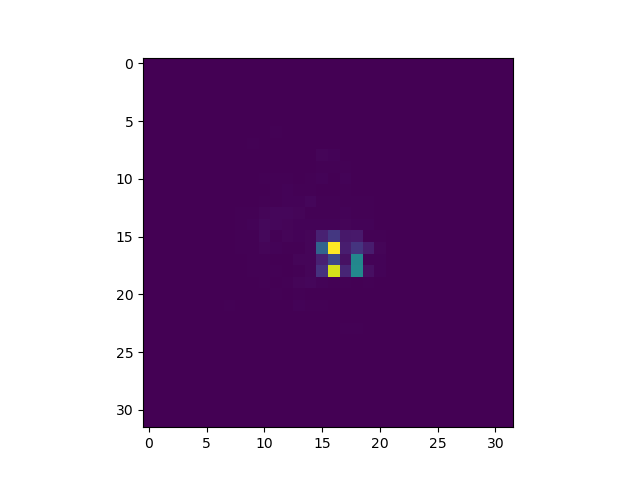
\includegraphics[width=.7\linewidth]{1450_poison_lrp.png}
			%\caption{Zugehörige Heatmap bezüglich der Klasse 'Höchstgeschwindigkeit: 80km/h'}
			
		\end{subfigure}
		\caption[(Optischer) Vergleich von korrumpiertem Datenpunkt und berechnter Heatmap.]{(Optischer) Vergleich von korrumpiertem Datenpunkt und berechnter Heatmap. Links: Verkehrsschild der Klasse 'Höchstgeschwindigkeit: 50km/h' versehen mit einem 3x3 Sticker und dem Label 'Höchstgeschwindigkeit: 80km/h'. Rechts: Zugehörige Heatmap bezüglich der Klasse 'Höchstgeschwindigkeit: 80km/h'.}
		\source{\cite{AC}}
		
		\label{vergleich_original_lrp}
	\end{figure}
	\subsection{Implementierungen}
	
	\subsubsection{Tensorflow}
	\subsubsection{pytorch}
	
	\textbf{Allgemeines Tutorial}:\footnote{\url{https://git.tu-berlin.de/gmontavon/lrp-tutorial}}\\ pytorch-LRP für VGG16 wird vorgestellt.\\
	
	
	\noindent \textbf{GiorgioML}\footnote{\url{https://giorgiomorales.github.io/Layer-wise-Relevance-Propagation-in-Pytorch/}}:\\
	Alternative pytorch-Implementierung basierend auf Tensorflow paper.\\
	
	\noindent \textbf{moboehle}\footnote{\url{https://github.com/moboehle/Pytorch-LRP}}:\\
	Der code entstand im Rahmen der Forschungsarbeit \cite{lrp_alzheimer}, in der eine Alzheimer-Festellung aufgrund von Bilddaten(scans?) vorgenommen wird. Framework leicht anpasspar. Benutzt pytorch hooks. 
	\noindent Unterstützte Netzwerkschickten\footnote{\url{https://github.com/moboehle/Pytorch-LRP/blob/master/inverter_util.py}}:\\
	\begin{comment}
	
	
	\noindent $allowed\_pass\_layers = (torch.nn.BatchNorm1d, torch.nn.BatchNorm2d,\\
	torch.nn.BatchNorm3d,
	torch.nn.ReLU, torch.nn.ELU, Flatten,
	torch.nn.Dropout,\\ torch.nn.Dropout2d,
	torch.nn.Dropout3d,
	torch.nn.Softmax,
	torch.nn.LogSoftmax,
	torch.nn.Sigmoid)$\\
	\end{comment}
	\begin{lstlisting}[language=Python, caption=Verfügbare Schichten und Aktivierungsfunktionen]
	torch.nn.BatchNorm1d, 
	torch.nn.BatchNorm2d
	torch.nn.BatchNorm3d,
	torch.nn.ReLU, 
	torch.nn.ELU, 
	Flatten,
	torch.nn.Dropout,
	torch.nn.Dropout2d,
	torch.nn.Dropout3d,
	torch.nn.Softmax,
	torch.nn.LogSoftmax,
	torch.nn.Sigmoid
	
	\end{lstlisting}
	\noindent \textbf{fhvilshoj}\footnote{\url{https://github.com/fhvilshoj/TorchLRP}}:\\
	
	
	
	\noindent LRP für linear und Convolutional layers
	
	\begin{itemize}
		\item Die Klassen
		
		torch.nn.Sequential, torch.nn.Linear und torch.nn.Conv2d werden erweitert, um autograd für die Berechnung der Relevanzen zu berechnen.
		
		\item Ausgabe der Relevanzen von Zwischenschichten ist möglich
		\item: Implementierte Regeln: epsilon Regeln mit epsilon=1e-1, gamma-regel mit gamma=1e-1. alphabeta-Reagel mit a1b0 und a2b1
		\item Netz muss hier umgeschrieben werden, sodass die Anwendung des Algorithmus möglich wird.
	\end{itemize}
	
	\begin{lstlisting}[language=Python, caption=Implementierte Regeln fhvilshoj]
	
	conv2d = {
	"gradient":             F.conv2d,
	"epsilon":              Conv2DEpsilon.apply,
	"gamma":                Conv2DGamma.apply,
	"gamma+epsilon":        Conv2DGammaEpsilon.apply,
	"alpha1beta0":          Conv2DAlpha1Beta0.apply,
	"alpha2beta1":          Conv2DAlpha2Beta1.apply,
	"patternattribution":   Conv2DPatternAttribution.apply,
	"patternnet":           Conv2DPatternNet.apply,
	}
	
	\end{lstlisting}
	
	\noindent \textbf{Zennit}:\footnote{\url{https://github.com/chr5tphr/zennit}}
	Zennit (Zennit explains neural networks in torch) 
	\begin{itemize}
		\item Modell wird mithilfe eines Canonizers so aufbereitet, dass LRP möglich wird
		\item Backward pass wird modifiziert, um Heatmaps zu erhalten.
		\item VGG- und ResNet-Beispiel
	\end{itemize}
	\section{Detektion von Poisoning-Angriffen basierend auf LRP} 
	In diesem Kapitel stellen wir das Verfahren vor, mit dem wir die Präsenz von Poisoning-Angriffen detektieren und die korrumpierten Datenpunkte aus dem Datensatz entfernen können.
	
	Die Idee besteht darin, ein kMeans-Clustering auf einer Klasse durchzuführen, die für verdächtig gehalten wird.
	
	Wichtig für das Clustering sind hierbei die Repräsentation der Daten, auf denen geclustert wird, sowie die Metriken, die eine Distanz und einen Mittelwertbegriff für mehrere Datenpunkte definieren.
	
	Als Repräsentation benutzen wir die Heatmaps, die mit der LRP, wie in \autoref{chapter_lrp} beschrieben, erzeugt werden.
	
	Für das kMeans-Clustering müssen wir im Vorfeld eine Clusteranzahl k fixieren und die Mittelpunkte der k Cluster initialisieren.
	
	In Lloyd's Formulierung \cite{lloyd1982least} wird mit einer gleich-verteilten zufälligen Initialisierung von $k$ Cluster-Zentren begonnen. Jeder Punkt im Datensatz wird anschließend dem nächstgelegenen Cluster-Zentrum zugeordnet. Für jedes Cluster wird anschließend ein neues Zentrum als Mittelwert berechnet.
	Diese beiden Schritte aus Zuordnung und Mittelpunktberechnung werden so lange wiederholt, bis sich die Cluster-Zentren nicht mehr ändern oder eine maximale Iterationszahl erreicht ist. Dieses Vorgehen wird als $k$-Means bezeichnet.
	
	Eine Variation des k-Means-Algorithmus, der sowohl die Laufzeit als auch die Genauigkeit verbessert, ist der sogenannte $k-means++$-Algorithmus \cite{kmeans++}. Dabei wird die Initalisierung in abgewandelter Form durchgeführt. Nach gleich-verteilter, zufälliger Bestimmung des ersten Cluster-Zentrums, werden die übrigen $k-1$ Zentren wie folgt gewählt:
	Die Wahl erfolgt proportional zur maximalen quadratischen Distanz zu allen vorher bestimmten Cluster-Zentren. Damit sind die Zentren so über den Datensatz verteilt, dass sie maximal weit auseinander liegen.
	
	Anschließend werden die im kMeans-Algorithmus üblichen Schritte aus Distanzberechnung und Mittelwert-Berechnung wiederholt.
	
	Dieses $kMeans++$-CLustering ist nochmals in 
	
	%TODO:kMeans-Algorithmus 
	
	zusammengefasst.
	
	
	Für die Bestimmung der Clusteranzahl k benutzen wir die Spektrale Relevanz-Analyse.
	
	
	
	
	\subsection{Idee}
	
	Die Idee zur Detektion von Poisoning-Angriffen besteht aus den folgenden Schritten:
	
	\begin{itemize}
		\item Berechnung der Heatmaps mithilfe der LRP
		\item Berechnung einer Distanzmatrix basierend auf $L^2-$ oder GMW-Distanz
		\item Spektrale Relevanzanalyse (Bestimmung der verschiedenen Cluster innerhalb einer Klasse)
		\item kMeans-Clustering zur Bestimmung der korrumpierten Datenpunkte
	\end{itemize}

	Diese werden wir im Folgenden näher betrachten.
	
	\noindent\textbf{Berechnung der Heatmaps mithilfe der LRP}.	Für die LRP wählen wir innmodel = InnvestigateModel(model.net, lrpexponent=2,
	method='e-rule', beta=0.5) und normalisieren die Heatmap anschließend.
	
	
	
	The theory of optimal transport generalizes thatintuition in the case where, instead of moving only one item at a time, one is concernedwith the problem of moving simultaneously several items (or a continuous distributionthereof) from one configuration onto another.\cite{computationalOT}
	\subsection{k-means / k-means++ -Clustering}
	Das k-means-Clustering gehört zu den unüberwachten Clustering-Verfahren. In der ursprünglichen Formulierung sind $n$ Datenpunkte $x_1,...,x_n \in \mathbb{R}^d$ und $k \in \mathbb{Z}_{>0}$ gegeben. Die Datenpunkte sollen so auf, die einzelnen Cluster verteilt werden, dass die $L^2$-Distanzen innerhalb eines Clusters zum Cluster-Zentrum minimal sind. 
	
	
	


	Baryzentrische Koordinaten \footnote{\url{https://de.wikipedia.org/wiki/Baryzentrische_Koordinaten}}
	
	\subsection{Spektrales Clustering}
	Wir folgen \cite{spectralClustering_tut}.
	Gegeben:Datenpunkte $x_i, ..., x_n$ sowie eine Größe $s = s_{ij} \in \mathbb{R}^{+}$, die einen paarweisen Zusammenhang der einzelnen Punkte beschreiben.
	
	Ziel: Aufteilen der Punkte in verschiedene Cluster, sodass sich Punkte innerhalb eines Clusters ähnlich bezüglich $s$ sind.
	
	Alternative Repräsentation der Daten mithilfe eines Ähnlichkeitsgraphen $G=(V,E)$ möglich.
	
	Umformulierung des Clustering-Problems mithilfe des Ähnlichkeitsgraphen: Finde Pertitionierung des Graphen, sodass die Kanten-Gewichte innerhalb einer Gruppe niedrig (niedriges Gesamtgewicht?) und außerhalb einer Gruppe große sind.\\
	
	
	Graph-Notationen:\\
	
	Verschiedene Konstruktionsmöglichkeiten von Ähnlichkeitsgraphen:
	
	\begin{itemize}
		\item $\varepsilon$-Nachbarschaft-Graph\\
		\item kNN-Graph\\
		\item fully connected graph
	\end{itemize}
	
	
	\subsection{Anwendung auf unterschiedliche Poisoning-Angriffe} \label{chapter_results} \label{chapter_experiments}
	\noindent \textbf{Berechnung der Relevanzen}:\\
	
	\noindent Wir berechnen die Relevanzen jedes einzelenen Eingabebildes klassenweise, d.h. besitzt eine Eingabe das Label y, so berechnen auf einem trainierten Netzwerk, für jeden Pixelwert der Eingabe, wie relevant dieser für die Ausgabe f(x) = y ist.\\
	Wir summieren über die Farbaxen des Bildes, um einzelne Relevanzen pro Pixelpunkt zu erhalten.\\
	Für die Berechnung der Relevanzen benutzen wir eine modifizierte Version des im Rahmen von \cite{lrp_alzheimer} entstandenen Programmcodes\footnote{\url{https://github.com/moboehle/Pytorch-LRP}}.\\
	\\
	\noindent \textbf{Vorverarbeitung der Relevanzen:}\\
	In \cite{unmaskingCH} wird anschließend ein Sum-Pooling auf die Relevanzen angewendet, um eine Dimensionsreduktion zu erhalten. Wie in \cite{imagenet_unhansed_v1} verzichten wir auf eine weitere Dimensionsreduktion, da wir nur relativ kleine Relevanzen der Größe $32x32$ verarbeiten.	\\
	
	Für eps=5e-2 liegen beide barycentren identisch weit weg. Probiere nun eps=5e-3
	
	\noindent \textbf{Berechnung der Distanzen und Aufstellen einer Affinitätsmatrix:}\\
	
	Wir berechnen zunächst eine Distannzmatrix, die die paarweisen Distanzen aller Heatmaps einer Klasse enthält.	
	
	Für die Berechnung der euklidischen Distanz betrachten wir Heatmaps $x,y$ der Größe $32x32$ als Elemente $x,y \in \mathbb{R}^{32*32}$ Die Distanz lässt sich dann wie in \autoref{l2dist} berechnen.\\
	
	Die Gromov-Wasserstein-Distanz lässt sich wie in \cite{gwd_averaging_kernels} angegeben berechnen. \\
	
	Barycenters Definition und Vergleich zum euklidischen Raum \cite{bary_wasserstein_space}
	
	In einer Affinitätsmatrix oder Ähnlichkeitsmatrik sind die \\
	
	\noindent \textbf{Berechnung Spektralen Einbettung:}\\
	
	\noindent \textbf{Dimensionsreduktion vor dem Clustering ?!}\\
	
	In \cite{AC} wird beispielsweise eine Dimensionsreduktion mit PCA durchgeführt.
	
	\noindent \textbf{k-Means-Clustering:}\\
	\begin{remark}
		In \cite{imagenet_unhansed_v1} Kapitel '2.3. Fisher Discriminant Analysis for Clever Hans
		identification' wird ein Verfahren vorgestellt, mit dem verdächtige Klassen indentifiziert werden können. Für diese würde man anschließend das obige Verfahren durchführen
	\end{remark}
	\subsection{Verwendete Distanzen \& Approximationen}
	Um die Struktur innerhalb einer Klasse zu analysieren, benötigen wir eine Metrik.
	Anhand dieser wird abhängig von den Heatmps einer Klasse eine Affinitätsmatrix berechnet, die dann anschließend zur Berechnung der Spektralen Einbettung als wichtigster Schritt von SpRAy verwendet wird. Wir wollen dazu die im Folgenden vorgestellten Metriken verwenden.\\
	Wie in \cite{imagenet_unhansed_v1} summieren wir über die Farbkanäle, um einen einzelnen Relevanzwert pro Pixelpunkt zu erhalten. Wir benötigen also eine Metrik zur Berechnung der Distanz zwischen 32x32 großen Heatmaps.\\
	Wir normalisieren die Relevanzen zusätzlich auf das Intervall $[0,1]$.\\
	Die Wahl der Pixel mit 99 Prozent der Gesamtmasse und anschließende Normalisierung wird vermutlich durchgeführt, um die Bedingung \autoref{eq:bed_mmspaces} zu erhalten.
	
	
	
	\newpage
	\appendix
	\section{Verwendete Netzwerke}
	
	Aufbau dieses Netzwerkes:
	1. Inception-Modul
	2. [pool1, batchConv1, pool2, batchConv2, pool3, batchConv3, pool4]
	3. Drei Lineare Schichten mit ReLu und Dropout dazwischen
	
	Im Unterschied zum offiziellen Inception Netz(v1v2v3) gibt es in dieser 
	vereinfachten Version keinen "stem" aus convs, 
	es geht direkt mit InceptionA los.
	
	Wie ähnlich sind sich InceptionA(hier) und das offizielle InceptionA-Modul?
	
	\section{Parameter für Training und Einlesen der Daten}\label{param_net}
	Die in \cite{CH} gewählten Parameter wären ein guter Ausgangspunkt.\\
	Für das Einlesen der Daten benutzen wir, sofern nicht weiter angegeben die folgenden Augmentierungen:
	
	\begin{lstlisting}[language=Python, caption=Augemntierung beim Einlesen der Daten]
	__train_transform = transforms.Compose(
	[
	transforms.RandomResizedCrop((image_size, image_size), 
	scale=(0.6, 1.0)),
	transforms.RandomRotation(degrees=15),
	transforms.ColorJitter(brightness=0.1, contrast=0.1, 
	saturation=0.1, hue=0.1),
	transforms.RandomAffine(15),
	transforms.RandomGrayscale(),
	transforms.Normalize(	mean=[0.485, 0.456, 0.406], 
	std=[0.229, 0.224, 0.225]),
	transforms.ToTensor()
	
	]
	
	
	
	\end{lstlisting}
	Die Werte von mean und std variieren für alle ausgeführten Poisoning-Angriffe. Anstatt beide jedes Mal erneut zu berechnen, verwenden wir die von pytorch angegebenen Werte \footnote{\url{https://github.com/pytorch/examples/blob/97304e232807082c2e7b54c597615dc0ad8f6173/imagenet/main.py\#L197-L198}}, die für die vor-trainierten Modelle empfohlen werden und auf dem Datensatz ImageNet\footnote{\url{https://image-net.org/}} basieren.\\ 
	Wir trainieren die Netzwerke über maximal 100 Epochen und benutzen \textit{early stopping} mit einer $patience=20$. Die verwendete Implementierung ist eine modifizierte Version von Bjarte Mehus Sunde \footnote{\url{https://github.com/Bjarten/early-stopping-pytorch}}, die wiederum auf PyTorch Ignite\footnote{\url{https://github.com/pytorch/ignite/blob/master/ignite/handlers/early\_stopping.pyt}} basiert.\\
	
	\section{Einlesen der Daten bei AC}
	Ohne Transformationen, wie den Testdatensatz.
	
	
	\section{Parameter für die ausgeführten Angriffe}\label{param_attacks}
	Für das projizierte Gradientenverfahren benutzen wir 10 Iterationen und eine Schrittweite von 0.015.
	
	\textbf{Label-konsistente Poisoning-Angriffe:}
	\section{Datensätze}
	GTSRB\footnote{\url{https://benchmark.ini.rub.de/gtsrb_dataset.html}}
	Datensatz Splitting (Train; Val, test)
	
	ImageNet besteht über 14 Millionen Bildern in 100 Klassen.
	\section{Programmcode}
	Der vollständige Programmcode ist verfügbar unter \url{https://github.com/lukasschulth/MA-Detection-of-Poisoning-Attacks}
	
	%\verbatiminput{Netlayout.txt}
	
	%\verbatiminput{InceptionNet3layout.txt}
	\section{Notizen}
	registered spaces \footnote{\url{https://arxiv.org/pdf/1809.06422.pdf}}
	Barycenters in the Wasserstein Space\footnote{\url{https://arxiv.org/pdf/1809.06422.pdf}}\\
	Was passiert bei der Kombination von 2 verschiedenen Triggern? Einmal keine Überlappung(d.h. 2verschiedene Trigger auf dem selben Bild) vs. auch beide Trigger auf einem Bild ist zulässig.
	\newpage
	
	\printglossaries
	
	\newpage
	
	\bibliographystyle{alpha}
	
	\bibliography{bibfileMAlukasschulth}
	
	
	
\end{document}
